\documentclass[11pt,reqno]{amsart}
\usepackage{xifthen,setspace}
\usepackage{hyperref}
   \topmargin=0in
   \oddsidemargin=0in
   \evensidemargin=0in
   \textwidth=6.5in
   \textheight=8.5in
\usepackage{pkgfile}
\newtheorem{setup}{Setup}
\newtheorem{assumption}{Assumption}
\newcommand{\PP}{\mathcal{P}}
\newcommand{\CC}{\mathcal{C}}
\newcommand{\e}{\varepsilon}
\newcommand{\dd}{\delta}
\allowdisplaybreaks


\newtheorem{claim}{Claim}
\newtheorem{theorem}{Theorem}
\newtheorem{proposition}{Proposition}
\newtheorem{lemma}{Lemma}
\newtheorem{corollary}{Corollary}
\newtheorem{prop}{Property}
\newtheorem{definition}{Definition}
\newtheorem{conjecture}{Conjecture}
\newcommand{\er}{{Erd\H{o}s-R\'enyi }}


\newcommand{\DD}{{\mathbb{D}}}
\newcommand{\sigmamin}{{\sigma_{\rm min}}}
\newcommand{\Bin}{{B_{\rm in}}}
\newcommand{\Bout}{{B_{\rm out}}}

\newcommand\moniker[1]{{\em (#1)}}
\newcommand\old[1]{}



\title{Recovery and Rigidity in a Regular Stochastic Block Model}

\author[Brito]{Gerandy Brito}
\address{Department of Mathematics, University of Washington}
\email{gerandy@math.washington.edu}

\author[Dumitriu]{Ioana Dumitriu}
\address{Department of Mathematics, University of Washington}
\email{dumitriu@math.washington.edu}

\author[Ganguly]{Shirshendu Ganguly}
\address{Department of Mathematics, University of Washington}
\email{sganguly@math.washington.edu}

\author[Hoffman]{Christopher Hoffman}
\address{Department of Mathematics, University of Washington}
\email{hoffman@math.washington.edu}

\author[Tran]{Linh V. Tran}
\address{International University, National University Hochiminh City}
\email{tvlinh@hcmiu.edu.vn}


\begin{document}

\maketitle
\begin{abstract}
The stochastic block model is a natural model for studying community detection in random networks.  Its clustering properties have been extensively studied in the statistics, physics and computer science literature.  Recently this area has experienced  major mathematical breakthroughs,  particularly for the binary  (two-community) version, see \cite{MNS12, MNS13, M13}.  
In this paper, we introduce a variant of the binary model which we call the regular stochastic block model (RSBM). We prove rigidity by showing that with high probability an exact recovery of the community structure is possible. Spectral methods exhibit a regime where this can be done efficiently. Moreover we also prove that, in this setting, any suitably good partial recovery can be bootstrapped to obtain a full recovery of the communities.
\end{abstract}


\section{Definition of the model and main results}
\label{definition}
The stochastic block model (SBM) is a classical cluster-exhibiting
random graph model that has been extensively studied, both empirically
and rigorously, across numerous fields. In its simplest form, the SBM
is a model of random graphs on $2n$ nodes with two equal-sized
clusters $\mathcal{A}$ and $\mathcal{B}$ such that
$|\mathcal{A}|=|\mathcal{B}|=n$ and $\mathcal{A} \cap \mathcal{B}
=\emptyset$. Edges between various pairs of vertices appear
independently with probability $p=p_n$ if the two vertices belong to the
same cluster and with probability $q=q_n$ otherwise.
Thus, for any vertex, the expected number of same-class neighbors is
$a:=a_n:=p (n-1) \sim pn$, and the expected number of across-class neighbors is
$b:=b_n:= q n$.

Given a realization of the graph, the broad goal is to determine
whether it is possible (with high probability) to find the partition
$\mathcal{A},\mathcal{B}$; and if the answer is yes, whether it is
possible to do so using an efficient algorithm. Otherwise, the best
one can hope for is the existence of an algorithm that will output a
partition which is highly  (or at least positively) correlated with
the underlying cluster. To this end, consider the space $\mathcal{M}$
of all algorithms which take as input a finite graph on $2n$ vertices and output a partition of the vertex set into two sets. 
Informally, we say that an algorithm in $\mathcal{M}$ allows for {\bf
  weak recovery} if, with probability going to $1$ as $n$ goes to infinity, it outputs a partition $(A',B')$ such that
$|\mathcal{A} \Delta A'|+|\mathcal{B} \Delta B'| =o(n)$  (here $\Delta$ denotes the symmetric difference).
We say that an algorithm allows for {\bf strong recovery} if, with
probability going to $1$ as $n$ goes to infinity, it outputs the
partition $(\A,\B)$. Finally, an algorithm in $\mathcal{M}$ will be called {\bf efficient} if its run time is polynomial in $n$.

The problem of community detection described above is closely related
to the min-bisection problem, where one looks for a partition of the
vertex set of a given graph into two subsets of equal size such that
the number of edges across the subsets is minimal. In general, this problem is
known to be NP-hard \cite{GJS76}; however, if the min-bisection is
smaller than most of the other bisections, the problem is known to be
simpler. This fact was noticed a few decades ago, with the advent of
the study of min-bisection in the context of the SBM. In particular, Dyer and Frieze \cite{dyer1989solution} produced one of the earliest results when they showed that if $p > q$ are fixed as $n \to \infty$ then the min-bisection is the one that separates the two classes, and it can be found in expected $O(n^3)$ time.
Their results were improved by Jerrum and Sorkin
\cite{jerrum1998metropolis} and Condon and Karp
\cite{condon2001algorithms}. Each of these papers were able to find
faster algorithms that worked for sparser  graphs. The latter work was
able to solve the min-bisection problem when the average degrees were
of order $n^{1/2+\epsilon}$. %For the case of finite average degrees, one of the best results is due to Boppana \cite{boppana1987eigenvalues}, who analyzed the min-bisection problem on a related model of random graphs.

Until a few years ago most of the literature on both the min-bisection
problem and community detection in the SBM had focused on the case of
increasing expected degrees (i.e.\ $a, b \to \infty$ as $n \to
\infty$), with the best results at that time showing that if the
smallest average degree is roughly $\log n$, then weak recovery is
possible (e.g., McSherry \cite{mcsherry2001spectral} showed that spectral clustering arguments can work to detect the clusters in this setting).
Recently, the sparse case, i.e. when $a, b=O(1)$ has been the focus of
a lot of interest.  This regime is interesting both from a theoretical
and an applied point of view since a lot of real world networks turn
out to be sparse; for more on this see \cite{DLLM08}. 
 Coja-Oghlan demonstrated a spectral algorithm that finds a bisection which is positively correlated with the true cluster when the average degree is a large constant \cite{coja2010graph}.
Using ideas from statistical physics, Decelle, Krzakala, Moore and Zdeborov\'a gave a precise prediction for the problem of recovering a partition positively correlated with the true partition in the sparse SBM \cite{decelle2011}. The prediction was rigorously confirmed in a series of papers by Mossel, Neeman and Sly \cite{MNS12} \cite{MNS13}, and Massouli{\'e}
  \cite{M13}, where it was shown that this level of recovery  is
  possible iff $(a-b)^2>(a+b)$. More recently, \cite{MNS14} found
  necessary and sufficient conditions for $a$ and $b$ under which
  strong recovery is possible. Before them, Abbe, Bandeira and
  Hall  \cite{abbe2014exact} also characterized strong recovery assuming the edge probabilities to be constant factors of $\frac{\ln(n)}{n}$.

In \cite{MNS12} Mossel, Neeman and Sly proposed two regular versions
of the SBM in a sparse regime, and they conjectured thresholds for the
recovery of a correlated partition for each of the models. They also suggested that spectral methods should help to differentiate between the regular SBM and a random regular graph. 
In this article we study a slightly different version of a regular SBM where in addition to the graph being regular,  the number of neighbors that a vertex has within its own community is also a constant. Formally, we have the following definition.
\begin{definition}\label{model}
For integers $n,d_1$ and $d_2$ denote  by $\mathcal{G}(n,d_1,d_2),$
the random regular graph with vertex set $[2n]$, obtained as follows:
Choose an equipartition (parts have equal sizes) $(\mathcal{A}, \mathcal{B})$ of the vertex set, uniformly from
among the set of such equipartitions. Choose two independent copies of uniform simple $d_1$-regular graphs  with vertex set $\mathcal{A}$, respectively $\mathcal{B}$. Finally, connect the vertices from $\mathcal{A}$ with those from $\mathcal{B}$ by a random $d_2$-bipartite-regular graph chosen uniformly. We refer to this family of measures on graphs as the regular stochastic block model (RSBM).
\end{definition}

The goal of this article is to investigate the similarities and
differences between the RSBM and the classical SBM. For the rest of
the article we assume that  $\min\{d_1,d_2\}\geq 3$.  This assumption
implies that, with high probability, the resulting graph is
connected. This differs from the SBM with bounded average degree,
which has a positive density of isolated vertices, which make strong recovery impossible. 
The  constant degree of all the vertices in the RSBM makes the local
neighborhoods easier to analyze; however, as this model lacks the edge-independence present in the SBM,  some computations become significantly more difficult. 

Throughout the rest of the article we say a sequence of events happen asymptotically almost surely (a.a.s.) if the probabilities of the events go to $1$ along the sequence. The underlying measure will be always clear from context.

Our first result, the next proposition, pertains to the rigidity of
RSBM; it says that the RSBM is asymptotically distinguishable from a uniformly chosen random regular
graph with the same average degree. Below, $||\cdot,\cdot||_{TV}$ denotes the total variation distance between measures.
\begin{proposition}\label{orthogonal}
Let $\mu_n$ be the measure induced by $\mathcal{G}(n,d_1,d_2)$ on the
set $\text{Reg}(2n,d_1+d_2)$ of all $(d_1+d_2)$-regular graphs on $2n$
vertices and let $\mu'_n$ be the uniform measure on the same set
$\text{Reg}(2n,d_1+d_2)$. Then for any positive integers $d_1, d_2
\geq 3$,
$$\lim_{n\to \infty} ||\mu'_{n},\mu_n||_{TV} = 1.$$ 
\end{proposition}
This result sharply contrasts the RSBM and the SBM (which is
indistinguishable from an \er random graph with the same size and
average degrees satisfying $(a-b)^2\leq (a+b)$ \cite{MNS12}).

In order to determine whether it is possible to recover the partition
in the RSBM, one must first answer a basic question about the random
graph $\mathcal{G}(n,d_1,d_2)$: is the `true partition' $(\A, \B)$ 
identifiable. I.e., is $(\A, \B)$ the only way to partition the graph such that the subgraphs on the parts are $d_1$-regular (which then implies that the subgraph across is $d_2$-bipartite)? The following result shows that the answer is yes if $d_1$ and $d_2$ are sufficiently large.  

\begin{theorem}\label{uniqueness}  
There exists a constant $d'>0$ such that, for $d_1>d_2>d'$, $\mathcal{G}(n,d_1,d_2)$ has a unique partition a.a.s.
\end{theorem}

The particular value of $d'$ that we get is far from optimal; we
conjecture that the conclusion of this theorem should be true for
$d'=2$. The proof of Theorem \ref{uniqueness} is quite technical and is given in section \ref{ortho}.
 
To our knowledge, this is the first uniqueness of partition result for
block models with constant degrees. Such a result is not true,
however, in the classical setting where the edges are independent, since with constant probability one has isolated vertices.

If the original partition is unique in most cases then one can, in principle, find the original partition by
exhaustive search, and hence achieve strong recovery. This is again in
sharp contrast with the SBM, where strong recovery is achievable only
in the case of growing degrees. 

The next natural direction is to look for an efficient algorithm for strong recovery. 
While we do not answer this question in general, we do exhibit one regime where such an algorithm exists. 
%The nature of the algorithm is essentially spectral. We believe that the regime defined below is the largest one can cover using properties of the graph's spectrum.



\begin{theorem}\label{str12}
Assume $(d_1-d_2)^2> 4(d_1+d_2-1)$ and $d_1$ is even. Then there is an efficient algorithm that allows strong recovery.
\end{theorem} 

 The reason for the above asumption on the parity of $d_1$ is that in this case our graph can be viewed as a ``random lifts", allowing us to exploit their spectral properties, see Section \ref{sop2}. 
%We will give the proof of Theorem \ref{str12} when $d_1$ is even in the main body of the text and postpone the proof for any value of $d_1$ to the appendix.

%The proof of the above theorem is broken into two parts. 
Nonetheless, we believe spectral arguments can be used to prove weak recovery, with no restriction on the parity of $d_1$, and record the following conjecture.  
\begin{conjecture}\label{weakpart1}
Assume  $(d_1-d_2)^2>4(d_1+d_2-1)$. Then there is an efficient algorithm that allows weak recovery.
\end{conjecture}

Having obtained weak recovery, one can then achieve strong recovery by recursively applying the majority algorithm where one simultaneously updates the label of each vertex by the majority label among the neighbors. That this can be done is again an example of the rigidity in this model, and highlights one of the main differences between RSBM and the classic SBM. It shows that for the former, existence of an efficient algorithm for weak recovery implies the existence of an algorithm for strong recovery. This contrasts with the separate thresholds in the SBM \cite{MNS14}.

We present the majority algorithm in the section below.

\subsubsection{Majority algorithm.}\label{ma1}
Recall that $\mathcal{A}$ and $\mathcal{B}$ are the true
communities. Let $(A,B)$ be any partition (not necessarily an
equipartition) of the vertex set. For each $i \in [2n]$, let $\sigma_i=+1$ if $i\in A$ and $\sigma_i=-1$ if $i\in B$. 
\begin{itemize}
 \item [] $\mathbf{Initialize}$ $A_0=A, B_0=B$.
 \item [] \textbf{For} $i\in [2n]$  (\text{majority rule})\\
									           $\hat \sigma_i=\text{sign}(\displaystyle{\sum_{v_j\sim v_i}\sigma_j})$
 \item[]	\textbf{Return} $A_1=\{v_i: \hat \sigma_i=+1\}$, $B_1=\{v_i: \hat \sigma_i=-1\}$		
\end{itemize}


Similar applications of the majority algorithm appear in \cite{abbe2014exact} and \cite{MNS14}. There, the authors find criteria for both weak recovery and strong recovery in the SBM. It is not hard to see that weak
recovery and strong recovery are not equivalent  in the sparse SBM,
since the presence of isolated vertices prevents strong recovery. 

%Throughout the rest of the article 
We will refer to the majority algorithm as \textbf{Majority}.
The following theorem yields strong recovery from weak recovery. %along with Lemma \ref{weakpart1}, completes the proof of Theorem \ref{str12}.

 \begin{theorem}\label{majority} Assume $d_1>d_2+4$.  Then there
   exists an $\e=\e(d_1)>0$  such that the following is true a.a.s.:
   given a graph $\mathcal{G}(n,d_1,d_2)$ and any partition $(A,B)$
   of its vertex set such that $|A\cap \mathcal{A}|>(1-\e) n$ and
   $|B\cap \mathcal{B}|>(1-\e) n$, \textbf{Majority} recovers the true
   partition $(\mathcal{A}, \mathcal{B})$ if started with $(A,B)$,
   after $O(\log(n))$ iterations. The constant in the $O(\cdot)$ depends on $\e, d_1.$
\end{theorem}

The way we iterate the \textbf{Majority} algorithm will be clear from the proof of Theorem \ref{majority}, see section \ref{proof_majority}.

\section{Main ideas and organization of the paper}\label{psk}

In this section we sketch the main ideas behind the proofs and also the structure of the paper.

\subsection{Organization}

There are five results we present in this paper. In section \ref{ortho}, we prove
Proposition \ref{orthogonal} and Theorem \ref{uniqueness}. This section also contains a review of some standard definitions in the random graph literature that we make use of throughout the paper. We present an informal sketch of the proof of Theorem \ref{uniqueness} in section \ref{uni}, introduce some useful notions on random lifts and multigraphs in section \ref{sop2}, where we explain how to obtain Theorem \ref{str12}. Section \ref{sec_weak}  is concerned with proving Theorem \ref{str12}, while section \ref{algorithm} contains the proofs of Theorem \ref{majority}.

% as well as Theorem \ref{str12} with no restriction on the parity of $d_1$. The proof of Lemma \ref{weakpart1} is deferred to the Appendix. 


\subsection{Sketch of the proof of Theorem \ref{uniqueness}.} \label{uni}
Recall from Definition \ref{model}, in the graph $G:=\mathcal{G}(n,d_1,d_2)$ on $[2n],$ $(\A,\B)$ form the true partition.

Let us introduce the following notation: for any $V\subset [2n]$ let $G_V$ denote the subgraph induced by $G$ on $V$. For disjoint subsets $V_1,V_2,$ let $G_{(V_1,V_2)}$ denote the subgraph on $V_1 \cup V_2$ induced by the edges in $G$ with one endpoint in $V_1$ and the other in $V_2.$
For any $v\in [2n]$ and $V \subset [2n]$ let $deg_V(v)$ denote the number of edges incident on $v$ whose other endpoint is in $V$.


Thus Theorem \ref{uniqueness} says that, a.a.s., there does not exist any $V\subset [2n]$ with $V\neq \A,\B$  and $|V|=n$ such that the following two conditions hold simultaneously:

\begin{itemize}
\item Both $G_{V}$ and $G_{[2n]\setminus V}$ are $d_1$-regular graphs.
\item $G_{(V,[2n]\setminus V)}$ is a $d_2$-regular bipartite graph.
\end{itemize}
 
However we show that it is even unlikely that  $G_{V}$ is
$d_1$-regular for any $V \neq \A,\B$ with $|V|=n$. 
To this end we fix such a $V$ and  let $V_1:=V\cap \A$, $V_2:=V \cap \B$, and assume $|V_2|=\alpha n$ with $\alpha \le \frac{1}{2}.$
Note that, given $G$, $V$ and $\A$, the degree sequence
$\{deg_{V_1}(v)\}_{v \in V_1}$ is determined; if $G_V$ were
$d_1$-regular graph then for each $v \in V$, $$deg_{V_1}(v)+deg_{V_2}(v)=d_1,$$ 
and hence the degree sequence $\{deg_{V_2}(v)\}_{v \in V_1}$ is also determined, i.e. the number of edges going from each vertex in $V_1$ to $V_2$ is fixed. 

It can be shown using the configuration model (see Section \ref{pm1}
for the definition) that the joint distribution of 
 $\{deg_{V_2}(v)\}_{v \in V_1}$ behaves like i.i.d.\
 $Bin(d_2,\alpha)$'s. The proof now follows by using the above to
 estimate the probability of a certain degree sequence from this
 distribution, and by a union bound over all possible choices of $V.$
We remark that the formal proof involves some case analysis depending on the size of $|V_2|$ and relies on the expansion properties of regular graphs when $|V_2|$ is small.  

\subsection{Sketch of the proof of Theorem \ref{str12}.} \label{sop2}

To prove Theorem \ref{str12}, we make use of the recent work on the spectra of random lifts of graphs in \cite{FK14,B15} and the references therein. For a wonderful exposition of lifts of graphs see \cite{Linial}. We now introduce the notion of lift of a multigraph.

\subsubsection{Random lifts and multigraphs}\label{rlmg}

By a multigraph we simply mean a graph that allows for multiple edges and loops. Next we define the notion of lift. Informally, an $n$-lift of a
multigraph $X=(V,E)$ is a multigraph $X_n=(V_n,E_n),$ such
that for each vertex in $V$ there are $n$ vertices in $V_n$ and
locally both graphs look the ``same''. Formally, let $V_n:=V \times
\{1,2,\ldots n\}$. To define the edge set
in the lift consider the set $S^{E}_n:=\{\pi_{e}\}_{e\in E}$ where
$\pi_{e}\in S_n$ (the set of permutations of $[n]$). We have:

 $$E_n:=\{((x,i),(y,\pi_{e}(i))): e=(x,y)\in E,\,\,\, 1\le i\le n\},$$
for $\pi\in S_{n}^{E}.$
Thus every edge in $E$ ``lifts'' to a matching in $E_n.$  For every $v \in V,$ let $v\times \{1,2,\ldots n\}$ be called the \emph{fiber} of $v.$

A random lift is the lift constructed from $\pi \in S_n^{E}$ where
$\{\pi_{e}\}_{e\in E}$ are chosen uniformly and independently from $S_n.$
Let $A$ and $A_n$ be the adjacency matrices of the multigraphs $X$ and $X_n$, respectively. One can check that all the eigenvalues of $A$ are also eigenvalues of $A_n$ and the corresponding eigenvectors can be ``lifted'' as well to an eigenvector (which is constant on fibers) of the lifted graph.
Let the remaining eigenvalues of $A_n$ be,
\begin{equation}\label{remain1}
|\mu_1| \ge |\mu_2|\ge \ldots \ge |\mu_{r}|,
\end{equation}
where $r=n|V|-|V|.$
With the above definitions we now state one of the main results in \cite{FK14}.
\begin{theorem}\label{spectralnorm} Let $d\ge 3$ be an integer and let $X$ be a finite, $d$-regular multigraph. If $X_n$ is a random $n$-lift of $X$ then, for any $\e>0,$ $$\lim_{n\to \infty}\P(|\mu_1|\ge 2\sqrt{d-1}+\e)= 0~.$$
\end{theorem}


Recall the definition of strong and weak recovery from Section \ref{definition}. We also  need the following definition. 
\begin{definition}\label{notlabel} Let $e:=e_{2n}$ be the vector of all ones of length $2n$. 
Also let $\sigma=\sigma_{2n}$ be the vector of signs which denotes the partition $\A,\B$ i.e. 
$$\sigma(x)=\left\{\begin{array}{cc}
+1 & x \in \A,\\
-1 & otherwise.
\end{array}\right.
$$
\end{definition}

The proof of Theorem \ref{str12} follows by first realizing the
graph $\cG(n,d_1,d_2)$ as a random lift and then using the above
theorem to show spectral separation of $A_n$; moreover, it can be
shown that, with high probability, $\sigma$ in Definition \ref{notlabel} is an eigenvector associated to the second eigenvalue of the lift. The proof of Theorem \ref{str12} is now reduced to finding a good approximation to the unitary eigenvector corresponding to the second eigenvalue. Note that this allows the strong recovery of the partition $(\A,\B)$.



\section{Proof of Proposition \ref{orthogonal} and Theorem \ref{uniqueness}.} \label{ortho}
Let $K_{n}$ be the support of $\mu_n$, i.e., $K_n$ is the set of all graphs which
are $d_1$-regular on $\mathcal{A}$ and $\mathcal{B}$ and $d_2$-regular
and bipartite across, for some equipartition $(\A, \B)$ of $[2n]$.
Let $|\mathcal{G}(n,d)|$  be the number of $d$-regular graphs on $n$ labelled vertices and let $|\mathcal{BG}(n,d)|$ be the number of $d$-regular bipartite graphs on $2n$ vertices. 
To show that $\mu'_n(K_n)\to 0$ we will use the following enumeration results that can be deduced from \cite{MWa03} and \cite{mckay1991asymptotic}. The idea is to count the number of points in the support of the measures $\mu_n$ and $\mu'_n$.
\noindent
We have from \cite[Corollary 5.3]{mckay1991asymptotic} :
\begin{equation}\label{regulargraph}
|\mathcal{G}(n,d)|=C \frac{(nd)!}{(nd/2)!2^{nd/2}(d!)^n}~,
\end{equation}
asymptotically in $n$, where $C=C(n,d)$ remains bounded as $n$ grows. Similarly, from \cite[Theorem 2]{MWa03}:
\begin{equation}\label{biregulargraph}
|\mathcal{BG}(n,d)|=C_1 \frac{(dn)!}{(d!)^{2n}}~,
\end{equation}
asymptotically in $n$, for $C_1=C_1(n,d)$ a bounded function. We have:
\[
\mu'_n(K_n)=\frac{|K_n|}{|\mathcal{G}(2n,d_1+d_2)|}
\]
To compute $|K_n|$, recall Definition \ref{model}, first choose $\mathcal{A}$ and then use \eqref{regulargraph} and \eqref{biregulargraph}. We get: 

\[
\mu'_n(K_n)=C_2{{2n}\choose{n}}\left(\frac{(nd_1)!}{(nd_1/2)!2^{nd_1/2}(d_1)!^n}\right)^2\frac{(nd_2)!}{(d_2)!^{2n}}
\]
\[
\times\frac{(n(d_1+d_2))!2^{n(d_1+d_2)}(d_1+d_2)!^{2n}}{(2n(d_1+d_2))!} 
\]
for $C_2=C_2(n,d_1,d_2)$ bounded as $n$ grows. Using Stirling's Formula we get:
\[
\mu'_n(K_n)= C_3\left(\frac{4{{d_1+d_2}\choose{d_1}}^2d_1^{d_1}d_2^{d_2}}{2^{d_1+d_2}(d_1+d_2)^{d_1+d_2}}\right)^n
\]
\[
= C_3\left(\frac{2{{d_1+d_2}\choose{d_1}}}{2^{d_1+d_2}}\right)^n\left(\frac{2{{d_1+d_2}\choose{d_1}}d_1^{d_1}d_2^{d_2}}{(d_1+d_2)^{d_1+d_2}}\right)^n
\]
Where $C_3$ equals $C_2$ times a universal constant. Both fractions on the right hand side above are less than $1$. This proves Proposition \ref{orthogonal}.
\qed

\subsection{Uniqueness of the clusters}\label{proofT1}

\subsection{Preliminaries}\label{pm1}
For the sake of completeness, we include in this section some of the basic definitions in the random graph literature. Specifically, we define the configuration model to sample random graphs and also the exploration process.
\subsubsection{Configuration model and exploration process}\label{ep1}
The configuration model, introduced by Bender and Canfield
\cite{bendercanfield} and made famous by Bollobas \cite{bollobas}, is
a well known model to study random regular graphs. Assuming that $dn$
is even, the configuration model outputs a $d$-regular  multigraph
with $n$ vertices. This is done by considering an array $\{\xi_{ij},
1\leq i\leq d$,~ $1\leq j\leq n\}$ and choosing a perfect matching of
it, uniformly among all possible matchings. A graph on $n$ vertices is
obtained by collapsing all $\xi_{ij}$ for $1\leq i\leq d$ into a
single vertex, and putting and edge between two vertices $j$ and $t$
for each pair $(\xi_{ij},\xi_{kl})$ present in the matching. We refer to the family $\xi_{ij}$ as \emph{half edges}. 

It is not hard to see that under the condition that the resulting graph is simple, the distribution of the graph is uniform in the set of all simple $d$-regular graphs. Furthermore, it is well known that, for any fixed $d$, as $n$ grows to infinity, the probability that a graph obtained by the configuration model is simple is bounded away from zero. More precisely, denoting by $G$ the resulting graph, one has (see \cite{bollobas}),
\[
\mathbb{P}(G\mbox{ is simple})=(1-o(1))e^{\frac{1-d^2}{4}}.
\]

Thus, to prove a.a.s. statements for the uniform measure on simple $d$-regular graphs it suffices to prove them for the measure induced on multigraphs by the configuration model.

One extremely useful property of this model is the fact that one can construct the graph by exposing the vertices one at a time, each time matching one by one the $d$ half edges of the correspondent vertex, to a uniformly chosen half edge among the set of unmatched half edges. This process will be used crucially in many of the estimates. We include the precise definition for completeness.  
\begin{definition}\label{conf_process}
Consider the following procedure to generate a random $d$-regular graph on $n$ vertices:
 \begin{itemize}
   \item[$-$] Fix an order of the vertices: $v_1< v_2<...< v_n$ and let $\Xi=\{\xi_{ij}\}, 1\leq i\leq d$ and $1\leq j\leq n$, be the set of half edges, where, for any $1\leq j\leq n$, $\xi_{ij}$ are the $d$ half edges incident to vertex $v_j$. Consider the usual lexicographic order on $\Xi$. 
 	 \item[$-$] Construct a perfect matching of $\Xi$ as follows:
           the first pair is $(\xi_{11},\hat{\xi})$ where
           $\hat{\xi}$ is chosen uniformly from $\Xi \setminus
           \{\xi_{11}\}$. Having constructed $k$ pairs, let
           $\xi_{ij}$ be the smallest half edge not matched yet, chose
           $\tilde{\xi}$ uniformly from the set of remaining unmatched
           half edges different from $\xi_{ij}$, and add the edge
           $(\xi_{ij},\tilde{\xi})$.
	 \item[$-$] Output a multigraph $G$, with vertex set $\{v_j\}$ and an edge set induced by the matching constructed in the previous step.
 \end{itemize}
\end{definition}

This construction outputs a graph with the same law as the one given by the configuration model. Conveniently, with this construction we discover all neighbors of vertex $v_1$ first, then we move to $v_2$ and expose its neighbors (it could be the case that some edges are connecting $v_1$ and $v_2$ and those were exposed before!) and so on.  We will refer to this procedure as the exploration process. 
All the above definitions can be easily adapted to  sample bipartite
regular graphs as well, and in this paper we will use both sets of definitions. 

\subsubsection{Proof of Theorem \ref{uniqueness}}\label{pou}

Recall that $d_1>d_2$ and that ($\mathcal{A}$,$\mathcal{B}$) are the true clusters. The idea, as discussed in Section \ref{psk}, will be to show that, conditioned on the choices of $\mathcal{A}$ and $\mathcal{B}$, if we choose another subset of $n$ vertices, the probability of having a $d_1$-regular graph on these $n$ vertices is small. The estimate on the above probability is crucial since it will then allow us to take a union bound over all possible subsets of size $n$ to conclude that, a.a.s., there is a unique pair of clusters.

First we need some definitions.
\begin{definition}\label{bdrydef}Given a graph $G=(V,E),$
\begin{itemize}
\item [i.]
For a vertex $v$ and a set of vertices $S$ denote by $deg_S(v)$ the number of neighbors of $v$ in $S$. 
\item [ii.]
For any subsets $V_1\subset V_2 \subset V$ define the boundary $\partial_{V_2}V_1$ to be the number of edges in $E$ whose one end point lies in $V_1$ and the other in $V_2\setminus V_1.$ 
When $V_2=V$  we use the simpler notation $\partial V_1.$
\end{itemize}
\end{definition}

Consider non-empty subsets $A\subset \mathcal{A}$, $B\subset \mathcal{B}$ such that $|A\cup B|=n$. Without loss of generality assume $|A|\ge|B|$ and let $\alpha$ be such that 
\begin{equation}\label{frac1}
\alpha n=|B|.
\end{equation}
 We will prove Theorem \ref{uniqueness} by showing that given the $d_1$-regular graph with vertex set $\mathcal{A}$, for any choice of $A$ and $B$ the probability that $A\cup B$ is a $d_1$-regular graph goes to zero as $n$ goes to infinity. We use the simple observation that since $\mathcal{A}$ is $d_1$-regular, to have $A\cup B$ $d_1$-regular, for any vertex $v \in A$, the number of neighbors of $v$ in $B$ must be equal to the number of neighbors of $v$ in $\mathcal{A}\setminus A.$ The technical core of the proof involves showing that the probability of this event is small.
 
 We start by proving a lemma. Recall that, in order to have a $d_1$-regular graph with vertex set $A\cup B$ with $A\subset \mathcal{A}$ and  $B\subset \mathcal{B}$ it is necessary that $deg_B(v)=deg_{\mathcal{A}\setminus A}(v)$ for all $v\in A$. For notational brevity let 
\begin{equation}\label{impnotation1} 
 g_v:=deg_{\A\setminus A}(v)
\end{equation} 
  for all $v\in A$. 
\begin{lemma} \label{constant1} Given  $A\subset \mathcal{A},B \subset
  \mathcal{B}$ and a sequence of non-negative numbers $g=(g_1,g_2,
  \ldots, g_{|A|})$ let $$p(g_1,g_2,\ldots,
  g_{|A|}):=\mathbb{P}(deg_B(v)=g_v~ \mbox{for all}~ v\in A).$$ Then,
  for any such $g$, $$\max_{g'} p(g'_1,g'_2,\ldots, g'_{|A|})=
  p(g^*_1,g^*_2,\ldots, g^*_{|A|}),$$ where $g^*_i\in\{\ell,\ell+1\}$
  for some non negative number $\ell=\ell(g)$. The maximum in the
  above is taken over all sequences $g'=(g'_1,g'_2,\ldots, g'_{|A|})$ such that $\sum_{i=1}^{|A|}g_i'=\sum_{i=1}^{|A|} g_i.$
\end{lemma}

The above lemma says that, given the total number of edges going from
$A$ to $B$, the probability of a possible degree sequence is maximized
when all the degrees are essentially the same. Clearly
$l=\left\lfloor{\frac{\sum_{i=1}^{|A|}g_{i}}{|A|}}\right\rfloor$; the
number of $(l+1)$ degrees occurring in $g^*=(g^*_1,g^*_2,\ldots,
g^*_{|A|})$ is determined by $\sum_{i}g^*_i=\sum_{i}g_i.$

\begin{proof} To compute $p(g_1,g_2,\ldots, g_{|A|})$ we use the exploration process for the $d_2-$regular bipartite graph $(\mathcal{A},\mathcal{B})$  where the vertices of $\mathcal{A}$ are exposed  one by one, as sketched in Subsection \ref{ep1}. We order the vertices so that the vertices of $A$ are exposed first. Let $\mathcal{F}_i$ be the filtration generated by the process up to the $i^{th}$ vertex.
Using the exchangeability of the variables $deg_{B}(v_i)$, given a
sequence $\{g_i\}$, w.l.o.g. we can assume $g_1=\min g_i$ and
$g_2=\max g_i$. 

Assume now $g_2-g_1>1$. We will show that $p(g_1,g_2,\ldots,
g_{|A|})<p(g_1+1,g_2-1,\ldots, g_{|A|})$, which implies the lemma. 
We start with the following simple observation:
\begin{align*}
\mathbb{P}(deg_B(v_i)=g_i,~i\geq3 ~ \big | ~\mathcal{F}_2, & deg_B(v_1)=g_1,~deg_B(v_2)=g_2) =\\ 
& \mathbb{P}(deg_B(v_i)=g_i,~i\geq3 ~ \big | ~\mathcal{F}_2, deg_B(v_1)=g_1+1,deg_B(v_2)=g_2-1).
\end{align*}
This is because under the above two conditionings the number of
remaining unmatched half edges in $A,\mathcal{A},B,\mathcal{B}$ is the same. 
Hence it suffices to show that 
\begin{align}\label{bayes}
\mathbb{P}(deg_B(v_1)=g_1, deg_B(v_2)=g_2)< \mathbb{P}(deg_B(v_1)=g_1+1, deg_B(v_2)=g_2-1).
\end{align}

Next we note that
\[
\mathbb{P}(deg_B(v_1)=g_1, deg_B(v_2)=g_2)~=~\binom{d_2}{g_1}\binom{d_2}{g_2}\frac{(\alpha nd_2)_{[g_1+g_2]}((1-\alpha)nd_2)_{[2d_2-g_1-g_2]}}{(nd_2)_{[2d_2]}},
\]
where $(x)_m$ is the falling factorial
$(x)_{[m]}=x(x-1)\ldots(x-m+1)$. To see the above, we first choose
those half edges of $v_1$ and $v_2$ that will connect to half edges in
$B$. Then we choose the $2d_2$ half edges in $\mathcal{B}$ that will
match with the corresponding half edges of $v_1$ and $v_2$ such that
exactly $g_1+g_2$ are incident on vertices in $B$. 

Substituting now into \eqref{bayes} we have:
\begin{align*}
p(g_1,g_2,...g_{|A|})< p(g_1+1,g_2-1,...g_{|A|}) &\Longleftrightarrow
\binom{d_2}{g_1}\binom{d_2}{g_2}< \binom{d_2}{g_1+1}\binom{d_2}{g_2-1}\\
& \Longleftrightarrow
(g_1+1)(d_2-g_2+1)< g_2(d_2-g_1)\\
& \Longleftrightarrow g_1-g_2+1<d_2(g_2-g_1-1)~,
\end{align*}
which follows immediately from $g_2>g_1+1$.
\end{proof}
\noindent

Recall that we are interested in the probability that $A\cup B$ is
$d_1$-regular for a fixed choice of $A$ and $B$. As already discussed, 
\begin{equation}\label{checkpoint}
\mathbb{P}(A\cup B~ \mbox{is $d_1$-regular})\leq \mathbb{P}(deg_{\mathcal{A}\setminus A}(v)=deg_B(v),\forall v\in A).
\end{equation}

Our next goal is to bound the probability of such an event. To this
end we recall the notion of stochastic dominance. 

Let  $\nu_1$ and $\nu_2$ be two probability measures on $\mathbb{Z}$,
and let $X \sim \nu_1,\,Y \sim \nu_2.$ We use $X \preceq Y$ to denote that $\nu_2$ stochastically dominates $\nu_1$. 

Recall now Definitions \ref{model} and \ref{bdrydef}, as well as
\eqref{impnotation1}.
\begin{lemma}\label{domination} Let $M=\min \{\partial_{\A} A,n/2\}$,
and let $Y=(Y_1,Y_2,\ldots, Y_{M})$ where $Y_i\sim Bin(d_2,2\alpha)$
are i.i.d.. Then
\[
\mathbb{P}(deg_B(v)=g_v~,~\forall\, v\in A~ \big |~\A) ~\le~ \prod_{i=1}^{M}\P(Y_i\ge 1)~.
\]
\end{lemma}  

For notational brevity, we have denoted by $\mathbb{P}(\cdot\mid \mathcal{A})$ the random graph measure $\mathcal{G}(n,d_1,d_2)$ conditioned on the subgraph induced by $\A$.
\begin{proof}
First recall that by Lemma \ref{constant1} the quantity on the left
hand side is maximized when for all $v$,  $g_v\in \{\ell,\ell+1\}.$ Hence we assume that this is the case.
Now to prove the lemma we consider the exploration process defined
above. The definition requires us to fix an order on the vertices of
$\mathcal{A}$; we do this in the  following way. Consider the  two cases: 
\begin{itemize}
\item [$i$.]$\ell=0:$
First come all the vertices $v_i \in A$ with $g_i=1$, followed by the remaining vertices in $A$. Then come all the vertices in $\mathcal{A}\setminus A$.
\item [$ii$.] $\ell>0:$
First come all the vertices $v_i \in A$ with $g_i=\ell$, followed by the remaining vertices in $A$. Then come all the vertices in $\mathcal{A}\setminus A$. 
\end{itemize}
Recall that $\mathcal{F}_i$ is the filtration up to vertex $i.$
Note that, for $1\leq i \leq \min (\partial_{\mathcal{A}} A,n/2)$, 
\[
deg_B(v_i) \big |\mathcal{F}_{i-1}~\preceq~Bin\left(d_2,\frac{\alpha nd_2-(i-1)}{nd_2-id_2}\right).
\]
This follows from the simple observation that for any of the cases
mentioned above for the $i^{th}$ vertex, there are at most $(\alpha
nd_2-(i-1))$ half edges in $B$ that haven't yet been matched. 
Now note that since by hypothesis $i\le \frac{n}{2},$
\begin{align*}
\frac{\alpha nd_2-(i-1)}{nd_2-id_2}& \le \frac{\alpha n d_2}{nd_2/2}\\
&= 2\alpha. 
\end{align*}
Thus we are done.
\end{proof}

As already used in the proof of the above lemma, 
\[
\mathbb{P}(A\cup B~\mbox{is $d_1$-regular}\mid \mathcal{A})\leq p(\ell,\ell,\ldots,\ell,\ell+1,\ldots,\ell+1)\] for some $\ell=\ell(\mathcal{A},A)$. 
\noindent
In case $i.$ we see that by Lemma \ref{domination}
\begin{align}
\label{exp1}
p(0,0,\ldots,0,1,\ldots,1)=p(1,1,\ldots, 1,0,\ldots,0) & \le \prod_{i=1}^{\min \{n/2,\partial_{\mathcal{A}}A\}}\mathbb{P}(Y_i\ge 1) \\
\nonumber 
& \le  \prod_{i=1}^{\min\{n/2,\partial_{\mathcal{A}}A\}} (2 d_2\alpha)
\end{align}
The first equality follows by exchangeability. The first inequality follows from Lemma \ref{domination}. The second is a simple consequence of the fact that for a nonnegative variable the probability of being bigger than $1$ is at most its expectation.

In case $ii$ by similar arguments 
\begin{align}
\label{exp2}
p(\ell,\ell,...\ell,\ell+1,...,\ell+1)&\le \prod_{i=1}^{n/2}\mathbb{P}(Y_i\ge 1)\\
\nonumber
& \le  \prod_{i=1}^{n/2} (2 d_2\alpha).
\end{align}
Note that in \eqref{exp2} the term $\partial_{\mathcal{A}}A$ does not appear. This is because in this case by hypothesis $$|\partial_{\mathcal{A}}A|\ge \ell |A|\ge \frac{n}{2}.$$
To proceed with the proof of Theorem \ref{uniqueness} we quote two standard results on the expansion of random $d$-regular graphs.
Let $\gamma$ be the spectral gap for the operator of the random walk in the uniform random regular graph $G\in \mathcal{G}(n,d)$, i.e.:
\begin{equation}\label{gapdef}
\gamma=1-\frac{\lambda_2}{d}
\end{equation}
where $\lambda_2$ is the second largest eigenvalue of the adjacency matrix of $G$.

\begin{theorem}\cite[Theorem 1.1]{F08} With probability going to $1$ as $n \to \infty,$ $$\gamma \ge 1-\frac{2}{\sqrt{d}}.$$
\end{theorem}
The next result was proven independently in \cite{LS88} and \cite{JS89}. We will use it as it appears in \cite[Theorem 13.14]{LPW}.
\begin{theorem}\label{min_cut} Let $G$ be a $d$-regular graph in $n$ vertices. For any $S \subset V(G),$ with $|S|\le \frac{n}{2},$
$$\frac{\gamma}{2}\le \frac{|\partial S|}{d|S|}.$$
\end{theorem}


Putting everything together we get the following:
For $d_1\ge 16$, a.a.s., for all $S\subset \mathcal{A} $ with $|S|\le \frac{n}{2}$ $$|\partial_{\mathcal{A}} S|\ge \frac{d_1}{4}|S|.$$
In particular since $|A|\ge n/2$ it follows that, a.a.s.,
\begin{equation}\label{expans1}
|\partial_{\A} A|=|\partial_{\A} (\mathcal{A}\setminus A)|~\ge~ \frac{d_1}{4}|\mathcal{A}\setminus A|.
\end{equation}

In case $i.$ ($\ell=0$) plugging \eqref{expans1} in \eqref{exp1} we get

\begin{align}\label{otra_exp}
\mathbb{P}(A\cup B~\mbox{is $d_1$-regular}| \mathcal{A}) &\le \prod_{i=1}^{\min(n/2,|\partial_{\A} A|)}\mathbb{P}(Y_i\ge 1) ~\le~ \prod_{i=1}^{\frac{|\partial_{\A} A|}{2}}\mathbb{P}(Y_i\ge 1)\\
\nonumber 
&\le \prod_{i=1}^{\frac{d_1}{8}\alpha n}\mathbb{P}(Y_i\ge 1)
\end{align}
assuming that the $d_1$-regular graph on $\mathcal{A}$ satisfies \eqref{expans1}. The second inequality follows from the simple observation that since $\ell=0,$  we have $|\partial A| \le n.$

Recall that we want an upper bound on the right hand side of \ref{checkpoint}. Combining Lemma \ref{domination}, \eqref{exp2} and \eqref{otra_exp} we get
\begin{align}\label{upbnd1}
\mathbb{P}(A\cup B~\mbox{is $d_1$-regular}\mid \mathcal{A})~\leq~  \mathbb{P}(Y\ge 1)^{\frac{d_1}{8}\alpha n}+\mathbb{P}(Y\ge 1)^{n/2}.
\end{align}
The two terms on the right hand side correspond to the two cases $\ell=0 $ and $\ell \ge 1$.

Next we show that the bounds in \eqref{upbnd1} are good enough to be able to use union bound over all possible choices of $A$ and $B.$ 
There are  $\binom{n}{\alpha n}^2$ ways to choose $A$ and $B$. Denote
by $R_{\alpha}$ the event that $A\cup B$ is $d_1$-regular for \textit{at least} one choice of $A$ and $B$. Thus by union bound,
\begin{align}\label{finalexp1}
\mathbb{P}(R_{\alpha})& \leq \binom{n}{\alpha n}^2\left[\mathbb{P}(Y\ge 1)^{\frac{d_1}{8}\alpha n}+\mathbb{P}(Y\ge 1)^{n/2}\right].
\end{align}

We now estimate the right hand side using Stirling's formula. 
Let $$H(x)=-x\log x-(1-x)\log(1-x)$$ be the binary entropy function. 
Then the two terms in the right hand side of \eqref{finalexp1}
are at most
$$\frac{2^{n[2H(\alpha)+\frac{d_1}{8}\alpha\log(\mathbb{P}(Y\ge 1))]}}{\sqrt{\alpha n}} \ \ \ \ \text{and} \ \ \ \ \frac{2^{n[2H(\alpha)+\frac{\log(\mathbb{P}(Y\ge 1))}{2}]}}{\sqrt{\alpha n}},$$
up to universal constants involved in Stirling's approximation. Our goal would be to upper bound the two exponents,
\begin{equation}\label{twocase1}
2H(\alpha)+\frac{d_1}{8}\alpha\log(\mathbb{P}(Y\ge 1))~~~\mbox{and}~~~2H(\alpha)+\frac{\log(\mathbb{P}(Y\ge 1))}{2}.
\end{equation}
Recall that $\alpha$ was defined in \eqref{frac1}.
Consider the three following cases:

\textbf{CASE $1$:} 
$\alpha \le \frac{1}{d^2_2}$.

In this case we will use the bound $\mathbb{P}(Y\ge 1)\le 2d_2 \alpha$  by Lemma \ref{domination}.
Plugging this in \eqref{twocase1} we get the following upper bounds 
$$2H(\alpha)+\frac{d_1}{8}\alpha\log(2d_2 \alpha)~~~\mbox{and}~~~2H(\alpha)+\frac{\log(2d_2 \alpha)}{2}.$$
Now,
\begin{align*}
2H(\alpha)+\frac{d_1}{8}\alpha\log(2d_2 \alpha)& =  -2\alpha \log(\alpha)+\frac{d_1}{8}\alpha\log(2d_2 \alpha) -2(1-\alpha)\log(1-\alpha)\\
&\le  \alpha \log(\alpha)(\frac{d_1}{32}-2)-2(1-\alpha)\log(1-\alpha)\\
& \le \alpha \log(\alpha)(\frac{d_1}{32}-4).
\end{align*}
To see the above inequalities first note that since $\alpha \le \frac{1}{d_2^2}$, $\log(2d_2 \alpha) \le \frac{\log(\alpha)}{4} $ as soon as $d_2\ge 4,$ and also $|(1-\alpha)\log(1-\alpha)|\le 4\alpha.$
Similarly for large enough $d_2$ we have 
\begin{align*}
2H(\alpha)+\frac{\log(2d_2 \alpha)}{2}& =  -2\alpha \log(\alpha)+\frac{\log( \alpha)}{8} -2(1-\alpha)\log(1-\alpha)\\
& \le \frac{\log( \alpha)}{16}~.
\end{align*}

Thus for large enough $d_2\le d_1$ $$\mathbb{P}(R_{\alpha})\le \frac{2^{3\alpha \log(\alpha)n}}{\sqrt{\alpha n}}. $$
Hence \begin{eqnarray}
\mathbb{P}\left(\bigcup_{\alpha\in I_1}R_{\alpha}\right)
 &\le& \sum_{\alpha\in I_1}\frac{2^{3\alpha \log(\alpha)n}}{\sqrt{\alpha n}}\nonumber \\
 &\le& n 2^{-3\frac{1}{n}\log(n)n} \nonumber \\ 
 &\le&  \frac{1}{n}, \label{pop}
\end{eqnarray}
where $\alpha\in I_1=(0,\frac{1}{d_2^2})$. The last term is derived using the following:
 The function $\alpha \log \alpha $ is decreasing from $0$ to $1/2$ and the least possible value of $\alpha=\frac{1}{n}$. Plugging this value of $\alpha$  we get the above. 

\textbf{CASE $2$:}  $\frac{1}{d^2_2}\le \alpha \le \frac{C}{d_2}.$ 

Now clearly in this range of $\alpha$, by stochastic domination $\mathbb{P}(Bin(d_2,\alpha)\ge 1)$ is maximized when $\alpha=\frac{C}{d_2}.$
We now use the Poisson approximation of $Bin(d_2,\frac{2C}{d_2})$ to bound the probability $\mathbb{P}(Y\ge 1)$ by a universal constant $c$ which is a function of $C$ for  all $\alpha $ in this range.
Using this, we rewrite \eqref{finalexp1} to get 
\begin{align*}
2H(\alpha)+\frac{d_1}{8}\alpha\log(c)&\le  -2\alpha \log(\alpha)+\frac{d_1}{8}\alpha\log(c) -2(1-\alpha)\log(1-\alpha)\\
&\le -4\alpha \log (\alpha)+\frac{d_1}{8}\alpha \log(c)\\
&\le -5\alpha 
\end{align*}  
for large enough $d_1.$
Similarly for large enough $d_2$ we have 
\begin{align*}
2H(\alpha)+\frac{\log(c)}{2}& \le \frac{\log(c)}{4}.
\end{align*}

Plugging in we get
\begin{align}\label{fexp1}
\mathbb{P}\left(\bigcup_{\alpha\in I_2}R_{\alpha}\right)\le \sum_{\alpha\in I_2}\frac{2^{-5\alpha n}}{\sqrt{\alpha n}}
& \le n 2^{-\frac{5}{d^2_2}n},
\end{align} 
where $I_2=[\frac{1}{d_2^2},\frac{C}{d_2}]$. 
Thus the proof for the case when $\alpha \le \frac{C}{d_2}$ is complete.

\textbf{CASE $3$:} $\frac{C}{d_2} \leq \alpha \leq \frac{1}{2}.$\\

We first need a preliminary lemma. For $d_2 \in \mathbb{N}$ and $\alpha \in (0,1)$ let $Z_{d_2,p}\sim Bin(d_2,p).$
\begin{lemma}\label{supbound}There exists a constant $C_1$ such that for all large enough $d_2$  
$$\sup_{p \in (\frac{C_1}{d_2}, \frac{2}{3}) }\sup_{1\le i\le d_2}\mathbb{P}(Z_{d_2,\alpha}=i)\le \frac{1}{400}.$$
 \end{lemma}
 
\begin{proof} It is a standard fact that for any $d_2,\alpha$
$$\sup_{1\le i\le d_2}\mathbb{P}(Z_{d_2,\alpha}=i) =\mathbb{P}(Z_{d_2,\alpha}=\lfloor{(d_2+1)\alpha \rfloor}).$$ 
Let $k=\lfloor{(d_2+1)\alpha \rfloor}.$
We now estimate $$\mathbb{P}(Z_{d_2,\alpha}=k)={d_2 \choose k} \alpha^{k}(1-\alpha )^{d_2-k}.$$ Since $k>C_1$ by hypothesis using Stirling's formula we have 
\begin{align*}
\mathbb{P}(Z_{d_2,\alpha}=k)&=O\left(\frac{1}{\sqrt{k}}2^{H(\alpha)d_2}2^{-H(\alpha)d_2}\right)\\
&=O\left(\frac{1}{\sqrt{C_1}}\right) \le \frac{1}{400} 
\end{align*}
 for large enough $C_1.$ 
\end{proof}
 
 
We now need another lemma. Consider the exploration process for
sampling the bipartite regular graph given by
$\mathcal{A},\mathcal{B}$ (sketched in  Definition
\ref{conf_process}), where vertices of $\mathcal{A}$ are exposed one
by one to find out the neighbors in $\mathcal{B}.$ We do this first
for each half edge incident to the vertices in $A$,  followed by the half edges corresponding to the rest of the vertices in $\mathcal{A}.$ Let us parametrize time by the number of half edges. Consider the Bernoulli variable
\begin{equation}\label{berno1}
B_t=\mathbf{1}(\mbox{the $t^{th}$ half edge is matched to a half edge in }B).
\end{equation}
Now note that the first $d_2$ half edges correspond to $deg_{B}(v_1),$ the second $d_2$ half edges correspond to $deg_{B}(v_2),$ and so on. 
We now make a simple observation that the Bernoulli probabilities do not change much from time $t$ to $t+d_2.$ This then shows that $deg_{B}(v_i)$ are essentially Binomial variables with probability depending on the filtration at time $(id_2).$
Formally, we have the following lemma: let $\mathcal{F}_i$ be the filtration generated up to time $(id_2)$ (when all the half edges up to vertex $i$ have been matched).
\begin{lemma}\label{totalvar1}For any $i\le \frac{n}{4}$ there exists a $p_i$ which is $\mathcal{F}_{i-1}$-measurable such that $$||deg_{B}(v_i)| \mathcal{F}_{i-1},Bin(d_2,p_i)||_{TV}= O\left(\frac{1}{n}\right),$$  where $||\cdot, \cdot||_{TV}$ denotes the total variation norm and the constant in the $O(\cdot)$ notation depends only on $d_2.$
\end{lemma} 
 
\begin{proof}To show this first note that the random variables $B_{t}$ in \eqref{berno1}  are Bernoulli variables with probability $$\hat p _t=\frac{\alpha n d_2 -\sum_{j\le t-1}B_j}{nd_2-t}~.$$  Then clearly   
for all $t\le \frac{nd_2}{4},$ $|\hat p _t-\hat p _{t-1}|\le \frac{4}{n}~.$
The proof thus follows since $$deg_{B}(v_i)=\sum_{(i-1)d_2<j\le id_2}B_j~.$$
\end{proof} 
\noindent
Recall $\ell$ from Lemma \ref{constant1}. Now suppose $A\cup B$ is $d_1-$regular. Then by definition 
\begin{align*}
\ell |A|\le \sum_{i=1}^{|A|}deg_{B}v_i\le d_2|B|& =\alpha n d_2 \\
\implies \ell \le \frac{\alpha}{1-\alpha}d_2 \le 2\alpha d_2.
\end{align*}
\noindent 
Using the above we get that for all $j\le \frac{n}{4}$:
\begin{equation}\label{lb1}
\frac{\alpha nd_2-j(\ell+1)}{nd_2-jd_2}\ge\frac{\alpha nd_2-\frac{n}{4}(3\alpha d_2)}{nd_2}\ge  \frac{\alpha}{4}.
\end{equation}

Above we used the fact that  $\ell+1 \le 2\alpha d_2+1\le 3\alpha d_2$ since $\alpha d_2>C>1$ by hypothesis. 
Also clearly for $j\le n/4$,  since $\alpha\le 1/2,$
\begin{equation}\label{ub1}
\frac{\alpha nd_2-j\ell}{nd_2-jd_2}\le 2/3.
\end{equation}
Assume that all the $deg_{B}(v_i)\in \{\ell,\ell+1\}.$ We have the following corollary.
\begin{corollary}\label{binomapprox}For all $1\le i\le n/4,$ if $deg_{B}(v_j)\in \{\ell,\ell+1\},$ for some $\ell \le 2d_2 \alpha$  for all $j\le i$ then there exists $p_{i}$ which is $\mathcal{F}_{i-1}$ measurable such that $$||deg_{B}(v_i),Bin(d_2,p_{i})||_{TV}= O\left(\frac{1}{n}\right)$$  where $\frac{\alpha}{4} \le p_{i}\le 2/3.$
\end{corollary}
\begin{proof}The proof is immediate from \eqref{lb1}, \eqref{ub1} and Lemma \ref{totalvar1}. 
\end{proof} 
We now complete the proof of Theorem \ref{uniqueness} in the case $\alpha\in I_3=[\frac{C}{d_2},\frac{1}{2}].$
Using the same notation we used before we have:
\begin{eqnarray}
\nonumber
\mathbb{P}\left(\bigcup_{\alpha\in I_3}R_{\alpha}\mid \A\right) & \le & \sum_{\alpha\in I_3}\sum_{A,B}\mathbb{P}(deg_B(v_i)=g_i)\\
\nonumber
& \le &\sum_{\alpha\in I_3} \binom{n}{\alpha n}^2 \frac{1}{400^{n/4}}\\
\nonumber
& = &\sum_{\alpha\in I_3} \frac{1}{{\alpha n}}2^{2H(\alpha)n}\frac{1}{400^{n/4}}\\
& \leq & n\frac{2^{2n}}{400^{n/4}}. \label{fexp2}
\end{eqnarray}
The first inequality is by the union bound. To see the second inequality observe first that by Lemma \ref{constant1} it suffices to assume that $g_i's \in \{\ell,\ell+1\}$. Thus the second inequality follows by Corollary \ref{binomapprox} and Lemma \ref{supbound} as soon as $$\frac{\alpha}{4}\ge \frac{C_1}{d_2}$$ which we ensure by choosing $C\ge 4C_1.$  

Thus combining \eqref{pop}, \eqref{fexp1} and \eqref{fexp2} we have shown that 
$$\mathbb{P}(\cup R_{\alpha}) \le \tau^{n}$$ for some $\tau=\tau(d_2)<1.$  
Hence we are done. 
\qed

\section{Theorem \ref{str12} and connection to the min-bisection problem}\label{sec_weak}

Throughout this section we always assume $d_1$ is even.
We first remark that, under the hypothesis of Theorem \ref{str12}, one can make a quick and simple
connection to the min-bisection problem. It turns out that, in the
case of the RSBM, the two problems are equivalent. More precisesly, in the proof of Theorem \ref{str12} below, we show that the second eigenvalue of $\mathcal{G}(n,d_1,d_2)$ equals $d_1-d_2$ with high probability, which implies that $\gamma=\frac{2d_2}{d_1+d_2}$ where $\gamma$ is the spectral gap defined in \eqref{gapdef}. Hence, it follows by Theorem \ref{min_cut}, that the size of the min bisection of $\mathcal{G}$($n,d_1,d_2$) is at least $n d_2$. Since the true partition $(\A,\B)$ matches this lower bound, it solves the min-bisection problem.

We now proceed towards proving Theorem \ref{str12}. 
%for $d_1$ even.  
 Recall the notion of random lifts from Section \ref{rlmg}.
We will now connect $\cG(n,d_1,d_2)$ (RSBM)  with random lifts of a certain small graph. 
Consider the following multigraph on two vertices: $u$ and $v$, with $d_2$ edges between $u$ and $v$ and $d_1/2$ self loops at both the vertices (recall that $d_1$ is even).
\begin{figure}[hbt]
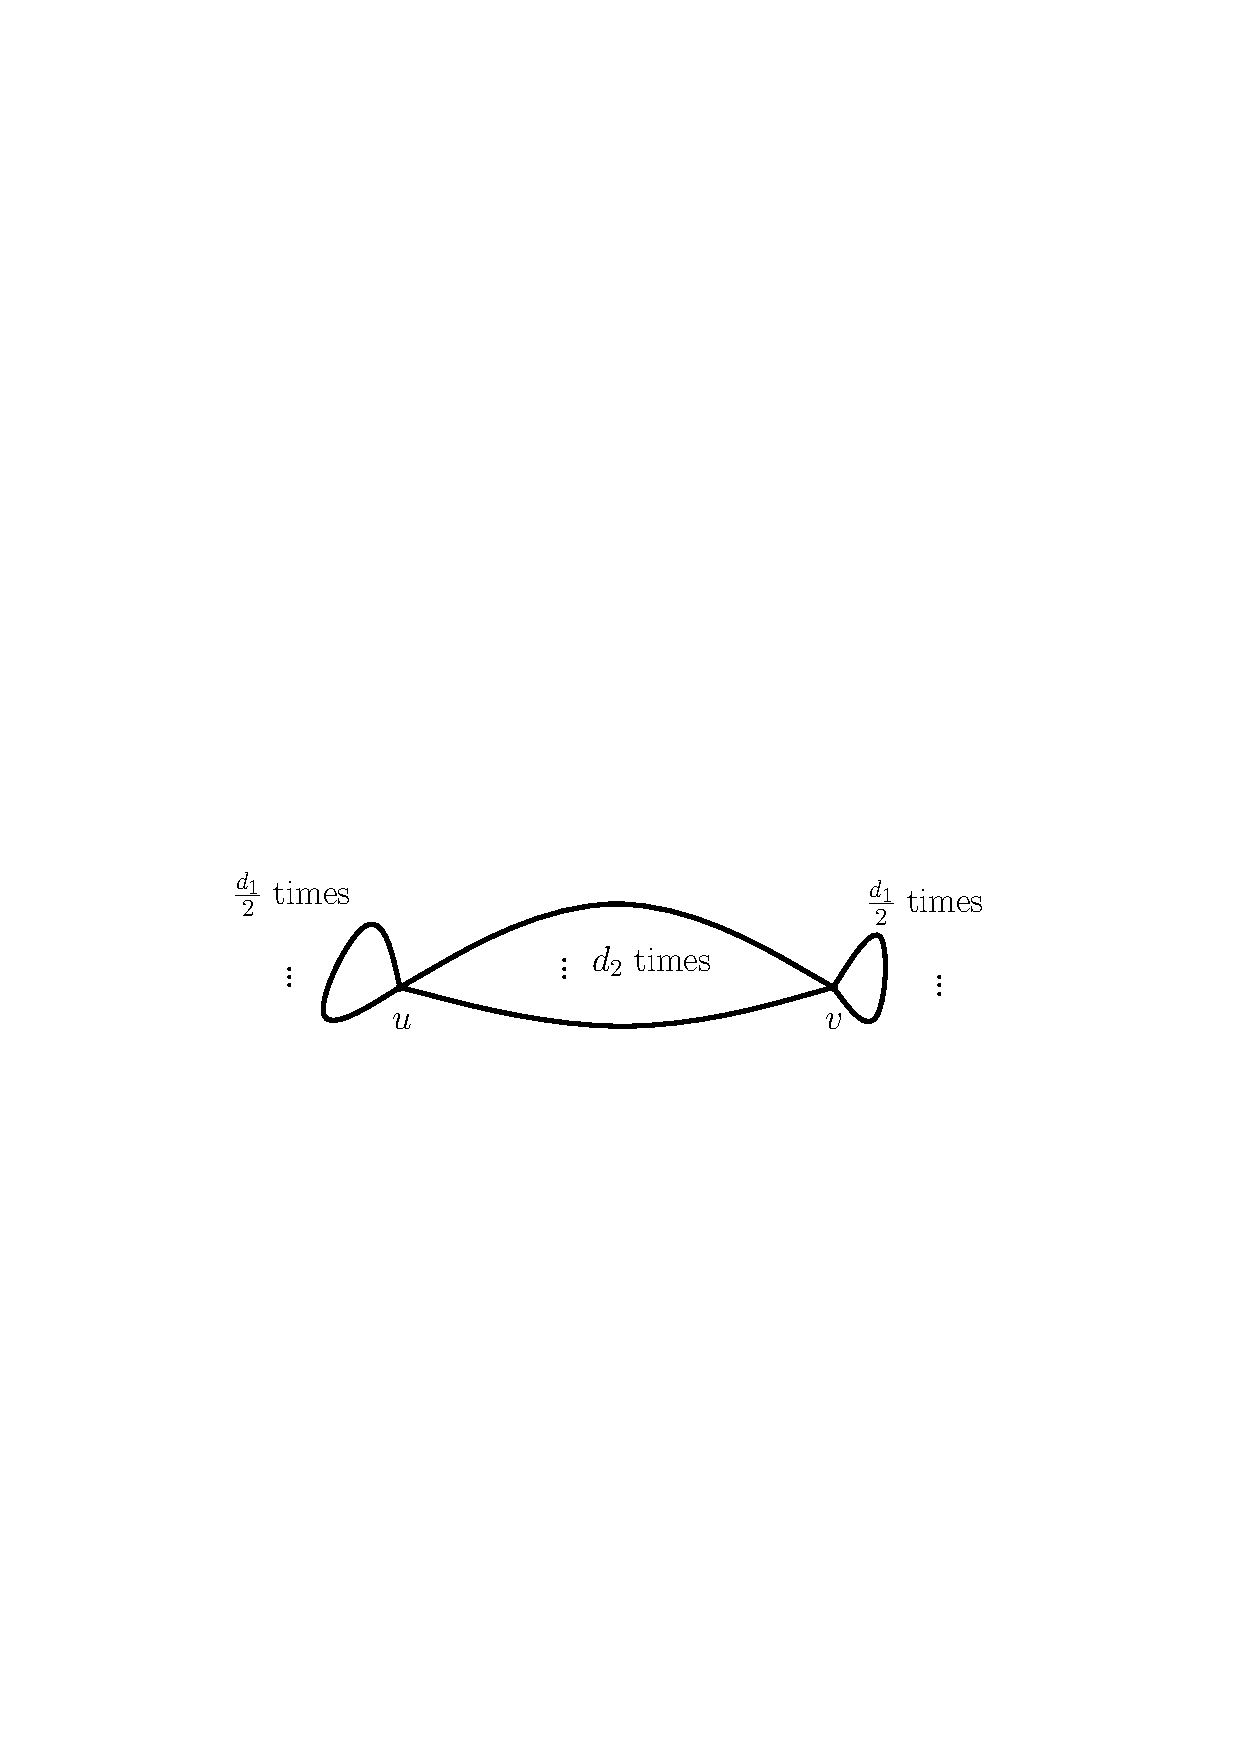
\includegraphics[scale=.8]{downstairs.pdf}
\caption{Multigraph lifting to $\cG(n,d_1,d_2)$.}
\label{down1}
\end{figure}
To randomly $n-$lift the above graph according to Section \ref{sop2} we choose uniformly $d_1+d_2$  many permutations: 
\begin{equation}\label{genperm1}
\pi_1,\pi_2,\ldots \pi_{d_1},\pi'_1,\pi'_2,\ldots \pi'_{d_2}
\end{equation}
 from $S_n.$

Let the lift be  $\sG(n,d_1,d_2)$ on the vertex set $\{u,v\}\times \{1,2,\ldots n\}$. We naturally identify it with $[2n]=\{1,2,3,4,\ldots 2n\}$ with the first $n$ numbers corresponding to $u\times \{1,2,\ldots n \}$ and the rest corresponding to $v \times \{1,2,\ldots n\}.$

Note that $\sG_1,$ the subgraph induced by $\sG(n,d_1,d_2)$ on $[n]$ has edge set $(i,\pi_{j}(i))$ for $i\in [n]$ and $j\in [d_1/2]$. Similarly $\sG_2,$ on $[2n]\setminus [n]$ has edges $(n+i,n+\pi_{j}(i))$ for $i\in [n]$ and $j\in [d_1]\setminus [d_1/2]$.
The edges between $[n]$ and $[2n]\setminus [n]$ are the edges $(i,n+\pi'_{j}(i))$ for $i\in [n]$ and $j\in [d_2].$
Recall $\cG(n,d_1,d_2)$ from Definition \ref{model}.  A standard model to generate regular graphs is the well known configuration
model, as also used in this article (see Section \ref{pm1})
Now notice that $\sG(n,d_1,d_2)$ is essentially the same as
$\cG(n,d_1,d_2)$ except the graphs are now generated using
permutations in \eqref{genperm1}.  This is known as the Permutation
model (see \cite{F08} and the references therein). 
We now use a well known result which says that the two models are
contiguous, i.e. any event occurring a.a.s. in one of the models occurs
a.a.s. in the other one as well (see \cite{GJKW02}).
\footnote{\cite[Theorem $1.3$]{GJKW02} actually shows contiguity of regular graphs under configuration model and the permutation model. Note that $\cG(n,d_1,d_2)$ and $\sG(n,d_1,d_2)$ are  constructed  from three independent regular graphs constructed using the configuration model and the permutation model. Since contiguity is preserved under taking product of measures, $\cG(n,d_1,d_2)$ and $\sG(n,d_1,d_2)$ are contiguous.}


We now prove Theorem \ref{str12}. Let the graph in Figure \ref{down1} be called $\sC$. The adjacency matrix of $\sC$ is $A_*:=\left[\begin{array}{cc}d_1 & d_2\\
d_2 & d_1 
\end{array}
\right]$ with eigenvalues $d_1+d_2$ and $d_1-d_2$ and corresponding eigenvectors $\left(\begin{array}{c}1\\
1 
\end{array}
\right)$ and $\left(\begin{array}{c}1\\
-1 
\end{array}
\right)$,
respectively. Let $A_{*,n}$ be the adjacency matrix of $\sG(n,d_1,d_2)$ which as discussed above is a random $n-$lift of $\sC.$ From the discussion in Section \ref{sop2} we have the following: 
\begin{itemize}
\item $d_1+d_2$ and $d_1-d_2$  are eigenvalues of $A_{*,n}$, with eigenvectors $e$ and $\sigma$ respectively (see Definition \ref{notlabel}). 
\item By Theorem \ref{spectralnorm}, for any $\e>0$, a.a.s., all the other eigenvalues $\lambda$ of $A_{*,n}$ satisfy $|\lambda|\le 2\sqrt{d_1+d_2-1}+ \e.$
\end{itemize}
Let $A_{n}$ be the adjacency matrix of $\cG(n,d_1,d_2).$ That the
first fact above holds for $A_n$ as well is easy to check. Moreover,
using the contiguity of the two models, $A_{n}$ also has the second
property a.a.s..
Note that  finding the partition $(\mathcal{A},\mathcal{B}),$ in  Definition \ref{model} is equivalent to finding $\sigma,$ (the eigenvector corresponding to the eigenvalue $d_1-d_2$). Now under the hypothesis of Theorem \ref{str12}, by the above discussion we see that $d_1-d_2$ is the second eigenvalue which is also separated from the first and rest of the eigenvalues. 
Thus, we can efficiently compute a unitary eigenvector, $w$, associated to this eigenvalue. To assign the communities, put $v\in \mathcal{A}$ if and only if $w_v>0$. Strong recovery is then achieved. This proves Theorem \ref{str12}.

\section{Complete reconstruction from partial reconstruction: proof of Theorem \ref{majority}} \label{algorithm}

In this section we prove Theorem \ref{majority}. The idea is to show
that, because of the rigid nature of the graph, if we initialize the
partition with a large number of vertices labeled correctly, one can
bootstrap to deduce the true labels of even more vertices in the next
step. We do this by looking at the majority of a vertex'
neighbors. Recall \textbf{Majority}  from Section \ref{ma1}. We prove
that with high probability the graph $\mathcal{G}(n,d_1,d_2)$ is such
that if the input $(A,B)$ has a large overlap with the true partition
$(\A,\B)$, then one round of the algorithm reduces the number of
wrongly labeled vertices by a  constant factor. Thus it follows then
that, with high probability, after $O(\log(n))$ iterations, no further corrections can be made
and the algorithm outputs the true communities. 


\begin{lemma}\label{maj_lem}  
Assume $d_1>d_2+4$ and let
$1/2<\lambda<1$. Then there exists an $\epsilon=\epsilon(d_1)>0$ such that, with probability
$1-O(n^{1/2-\lambda})$, the graph has the property that if  $(A,B)$ (the input)  satisfies $\min\{|A\cap \mathcal{A}|,|B\cap
\mathcal{B}|\}>(1-\epsilon)n$ and if $|\mathcal{A}\bigcap B|=:k$ and $|\mathcal{B} \bigcap A|=:k'$, then 
\[
|\mathcal{A}\bigcap B_1|\leq \lambda  k~\mbox{and}~
|\mathcal{B}\bigcap A_1|\leq \lambda k'~.
\] 
where $(A_1,B_1)$ is the output after one round of \textbf{Majority}.
\end{lemma}
The constant in $O(\cdot)$ depends on $d_1,\lambda, \epsilon.$

\begin{proof}
Let $v \in \mathcal{A}\bigcap B_1$ (that is, $v$ has the
wrong label after one iteration of \textbf{Majority}). We claim that $v$ has more than two neighbors in $\mathcal{A}\bigcap B$, otherwise $v$ will have at least $d_1-2$ neighbors in $\mathcal{A}\bigcap A$ and hence its label will be the sign of:
\[
\sum_{i\sim v} \sigma^1_i\geq d_1-2-(d_2+2)> 0~,
\] 

which contradicts the assumption that $v\in
\mathcal{A}\bigcap {B}_1$. 
Thus the occurrence of the event $\left | \mathcal{A}\bigcap {B}_1
\right | \geq \lambda k$ implies the occurrence of the event
\begin{center}
$E_k:=\{\exists \text{ a subset } S \subset \mathcal{A}, ~ |S|=\lambda k:  \mbox{ any } v\in S \mbox{ has at least three neighbors in}~ \mathcal{A}\bigcap B\}~.$
\end{center}

Hence an upper bound on the probability of the event $E_k$ will be an upper
bound on the failure probability for \textbf{Majority} to reduce
the size of the set of incorrectly labeled vertices in $\mathcal{A}$
by a fraction $1- \lambda$. 

We compute now an upper bound on the probability of $E_k$. 
By the exploration process (see Definition \ref{conf_process})  it follows that 
for vertices in the set $S$, the degree sequence $\{deg_{(\mathcal{A}\bigcap B)}(v)\}_{v \in S}$  is
stochastically bounded by a vector of i.i.d.\ binomial random
variables $\{Z_v\}_{v \in S}$, i.e.,
\[
\{deg_{(\mathcal{A}\bigcap B)}(v)\}_{v \in S} \preceq \{Z_v\}_{v \in S} ~, ~~\mbox{where}~ Z_v ~ {\sim}
~ Bin(d_1,\frac{k}{n-\lambda k})~.
\]
By stochastic domination of vectors we mean the existence of a coupling of the two distributions such that the one vector is pointwise at most the other vector. 
As $\P(Z_v\geq 3)\leq \left(\frac{d_1k}{n-\lambda k}\right)^3$, by
union bound and counting the number of choices for all the possible sets
$\mathcal{A}\bigcap B$ of size $k$ and $S$ of size $\lambda k$, we obtain
the following:
\[
\P(E_k)\leq \binom{n}{k}\binom{n}{\lambda k}\Big(\frac{d_1k}{n-\lambda k}\Big)^{3\lambda k}~.
\]


Adding over all possible $k$, we obtain
\begin{eqnarray} \label{bound1}
\P\left( \left | \mathcal{A}\bigcap {B}_1 \right | \geq \lambda
k~|~k\leq \epsilon n \right)& \leq & \sum_{k=1}^{\epsilon
  n}\binom{n}{k}\binom{n}{\lambda k}\Big(\frac{d_1k}{n-\lambda
  k}\Big)^{3\lambda k} \\
 &\leq & \sum_{k=1}^{\epsilon n} \Big(\frac{d_1^{3\lambda}e^{1+\lambda}}{\lambda^{\lambda}(1-\lambda)^{3\lambda}}\Big)^k\Big(\frac{k}{n}\Big)^{(2\lambda-1)k}
\end{eqnarray}
The last inequality follows by using the bound
$\binom{n}{m}\leq\Big(\frac{ne}{m}\Big)^m$, as well as the fact that
$n - \lambda n \leq n - \lambda k$. 
Denote now by $c= c(d_1) :=\frac{d_1^{3\lambda}e^{1+\lambda}}{\lambda^{\lambda}(1-\lambda)^{3\lambda}}$.

We show now that the sum in \eqref{bound1}   is $O(n^{1/2-\lambda})$. We split this sum into two parts,
$P_1$ and $P_2$, the first representing the sum of all the terms corresponding to indices up to $\lfloor \sqrt{n} \rfloor$, and the second part
representing the rest. For $P_1$, we obtain that 
\begin{eqnarray*}
P_1 & = & \sum_{k=1}^{\lfloor \sqrt{n} \rfloor} c^k
\Big(\frac{k}{n}\Big)^{(2\lambda-1)k}\leq \sum_{k=1}^{\lfloor
  \sqrt{n} \rfloor}
c^k n^{-(\lambda-1/2)k}\\
&  \leq & \sum_{k=1}^{\infty} \left (
  \frac{c}{n^{\lambda - 1/2}} \right)^k \\
& \leq & \frac{2c}{n^{\lambda-1/2}}~.
\end{eqnarray*}
The last inequality is true for large $n$. To bound $P_2$, we note that $k/n \leq \epsilon$ and we write: 
\[
P_2 = \sum_{k=\lceil \sqrt{n} \rceil}^{\epsilon n}
c^k\Big(\frac{k}{n}\Big)^{(2\lambda-1)k}\leq \sum_{k=\lceil \sqrt{n}
\rceil}^{\infty} (c\epsilon^{2\lambda-1})^k\leq
\frac{1}{1-c\epsilon^{2\lambda-1}}(c\epsilon^{2\lambda-1})^{\lceil
  \sqrt{n} \rceil}.
\] 
The last inequality above follows by choosing $\epsilon$ so that $c \epsilon^{2 \lambda-1}
<1$. 
Hence the probability of event $E_k$ is $O
\left(n^{1/2 -\lambda}\right).$
As the problem is symmetric in $\mathcal{A}$ and $\mathcal{B}$, it
follows that a similar bound can be found for the event that
$|\mathcal{B} \bigcap A_1| > \lambda k'$. Thus by union bound,
the probability of both events is also $O\left(n^{1/2 -\lambda}\right)$,
 and the proof of the lemma is complete.
\end{proof}

\subsection{Proof of Theorem \ref{majority}}\label{proof_majority}
Let $\epsilon=\epsilon(d_1)$ as in Lemma \ref{maj_lem}. Initialize \textbf{Majority} as $({A}_0,{B}_0)=(A,B)$ where $A, B$ satisfy the conditions of Lemma \ref{maj_lem}. Denote by $({A}_i,{B}_i)$ the partition after the $i^{th}$ iteration of \textbf{Majority} where $A_i$ corresponds to the vertices labeled $+1$, i.e., $(A_i,B_i)$ is the output of the algorithm when we initialize it with $({A}_{i-1},{B}_{i-1})$.
Consider the random variables
$
X_i=\max\{ |\mathcal{A}\bigcap {B}_i|;|\mathcal{B}\bigcap {A}_i|  \}.$
Note that $\{X_i=0\}$ iff $\mathcal{A}={A}_i$ (and thus
$\mathcal{B}={B}_i$). Also by the hypothesis $X_0 \le \e n,$ so Lemma \ref{maj_lem} implies that
\[
\P(X_i\leq \lambda^i k~,\forall~ 1 \leq i )\geq 1-O(n^{1/2-\lambda}).
\]

Let now $t=\left\lceil \frac{\log(\epsilon n)^{-1}}{\log{\lambda}}
\right\rceil$. 
 Since the $X_i$s  are integer-valued random variables, we have
\[
\P(X_t=0)\geq 1-O(n^{1/2-\lambda})~,
\] 
which proves the theorem.
\qed

%\noindent \textbf{Proof of Theorem \ref{str12}.} The proof is a straightforward corollary of Lemma \ref{weakpart1} and Theorem \ref{majority}.
%\qed


\noindent {\bf Acknowledgments} 
We thank Charles Bordenave for pointing out to us the connection between random lifts and the RSBM. ID acknowledges support from NSF grant DMS-08-47661. CH acknowledges support from NSF grant DMS-1308645 and NSA grant H98230-13-1-0827. GB and SG were partially supported by NSF grant DMS-08-47661 and NSF grant DMS-1308645.

\nocite{}
\bibliography{rsbm}{}
\bibliographystyle{plain}


\end{document}

%%%%%%%%%%%%%%%%%%%
% Appendix 
%%%%%%%%%%%%%%%%%%%

\section{Appendix: Proof of Lemma \ref{weakpart1}}\label{pow1}
Recall that we have used spectral properties of random lifts to prove Theorem \ref{str12} when $d_1$ is even, see section \ref{sec_weak}. The general proof relies on studying the matrix of self-avoiding walks (formally defined below)   of the
graph $\mathcal{G}$($n,d_1,d_2$). This is the same matrix used in
\cite{M13} to prove the blockmodel threshold conjecture. 
This section adapts the techniques in that paper to the regular setting to prove Lemma \ref{weakpart1}. 

In the case of the RSBM, the lack of edge independence increases the
complexity of many of the calculations.  On the other hand, the rigid nature of the model forces certain other calculations to be much
easier  for e.g. the size of small neighborhoods.  

The key ingredient in the proof of Lemma \ref{weakpart1} will be Proposition \ref{spectral}. Its proof hinges on two
technical lemmas we present below. We give here the proof of
Proposition \ref{spectral}, subject to these two lemmas, whose proofs
we defer to Sections \ref{neigh} and \ref{spec}. 

Let us recall the definition of a self-avoiding walk on a graph
$G$. Given two vertices $i$ and $j$ and a length $l>0$, a self-avoiding walk from $i$ to
$j$ of length $l$ is a graph path $(i=v_{0},v_{1},...,v_l=j)$ such
that $|\{v_{0},v_{1},...,v_{l-1}\}|=l$.

We denote by $S^{(l)}$ the matrix whose entry $S^{(l)}_{ij}$ equals
the number of self-avoiding walks of length $l$ between $i$
and $j$, for all $1 \leq i,j \leq 2n$.

\begin{definition}\label{aligned}
We say that the sequence of unitary vectors $\{ v_n \}_{n \geq 1}$ is
asymptotically aligned with the sequence of unitary vectors $\{ w_n \}_{n \geq
  1}$ if:
\begin{eqnarray} \label{alignment}
\lim\limits_{n \rightarrow \infty} |<v_n,w_n>|& =& 1.
\end{eqnarray}
\end{definition}
Definition \ref{aligned} means that, asymptotically, $v_n$ and $w_n$ are the same up to a factor of $-1$. 
Throughout the rest of the article let
\begin{equation}\label{eigennotation}
\lambda_1 \geq \lambda_2 \geq \lambda_3 \geq \ldots \geq
\lambda_{2n}
\end{equation}

 be the eigenvalues of $S^{(l)}$,

\begin{proposition}\label{spectral}
Assume $(d_1-d_2)^2>4(d_1+d_2-1)$. Let $l= c \log(n)  $
where $c$ is a constant such that $c \log(d_1+d_2)< \frac{1}{4}$. For any fixed $ \e >0$ the
following three events happen with high probability as $n$ grows:
 \begin{itemize}
  \item[(a)] $\lambda_1 = (d_1+d_2)(d_1+d_2-1)^{l-1} + o(1)$ and any unitary eigenvector associated
    to $\lambda_1$ is asymptotically aligned with $e$ (the vector of
    all ones). 
	\item[(b)] There exists a constant $A>0$ such that $ \lambda_2
          = A \alpha^l (1+o (1))$, where $$\alpha =
          \frac{d_1-d_2 + \sqrt{(d_1 - d_2)^2 - 4(d_1+d_2-1)}}{2}~;$$ any unitary
            eigenvector associated to $\lambda_2$ is asymptotically
            aligned with $\sigma$ (the vector of labels). 
	\item[(c)] $|\lambda_k| \leq |\lambda_3|
          \leq n^{\epsilon}(d_1+d_2)^{l/2}(1+o(1))$, for all $3 \leq k
          \leq 2n$. 
 \end{itemize}
\end{proposition}

\begin{remark} Note that as $(d_1 - d_2)^2 > 4(d_1+d_2-1)$, 
\[
d_1 - d_2 +\sqrt{(d_1-d_2)^2 - 4(d_1+d_2-1)} \geq d_1 - d_2 + 1
>2\sqrt{d_1+d_2-1}+1> 2 \sqrt{d_1+d_2}~,
\]
the latter inequality being true as $d_1+d_2\geq 6$. This, in turn, means that
\begin{eqnarray} \label{sep}
\alpha & = & \frac{d_1-d_2+\sqrt{(d_1-d_2)^2 -4(d_1+d_2-1)}}{2} >
  \sqrt{d_1+d_2}~,
\end{eqnarray}
and as $l = O(\log n)$, by picking $0<\epsilon< 1
- 4c \log(d_1+d_2)$, \eqref{sep}
is enough to show that $\lim\limits_{n \rightarrow \infty}
|\lambda_3|/|\lambda_2|= 0$, so the first two eigenvalues of $S^{(l)}$
are separated from the bulk. Also note that $\alpha < d_1-d_2 < d_1+d_2-1$,
so $\lambda_1$ and $\lambda_2$ are also separated from each other.\end{remark}

From part $(b)$ of Proposition \ref{spectral} one can see how to construct a labeling that recovers at least
$(1-\epsilon)n$ vertices correctly, for any $\epsilon>0$ and $n =
n(\epsilon)$ large enough using an eigenvector associated to the second eigenvalue.


In order to understand the nature of the neighborhoods of
$\mathcal{G}(n, d_1, d_2)$, we will need the fact that cycles are few and far from each other,
with high probability. To this end, we introduce the notion of
\emph{tangle-freeness}, which by now is a standard concept in the random graph literature. For e.g. see  \cite{F08} and \cite{LS10}. 

For a vertex $v$ in $\mathcal{G}(n,d_1,d_2)$, and for $t \in
\mathbb{N}$ let the ball of size $t$ centered at $v$ be denoted by
\[
B_t(v)=\{u \in \mathcal{G}(n,d_1,d_2): d(u,v)\leq t\}~,
\]
where $d(u,v)$ is the graph distance between vertices $u$
and $v$. We define the  boundary of $B_t(v)$ by
\[
\partial B_t(v)=\{u\in \mathcal{G}(n,d_1,d_2): d(u,v)=t\}~.
\]

\begin{definition}
A graph G is said to be \textit{l--tangle--free} if for any vertex $v$
in $G$ the ball $B_l(v)$ contains at most one cycle. 
\end{definition}

As we will see, with probability going to $1$ the random graph $\mathcal{G}(n, d_1, d_2)$  is 
$l$--tangle--free for $l = c \log n$ for a small enough constant $c$ (the $c$  in the statement of Proposition \ref{spectral} works). 

The next  two  lemmas contains estimates for the leading two eigenvalues and the corresponding eigenvectors which imply spectral separation. The proofs we defer to the next
sections. 

\begin{lemma}\label{top eigenvalues}
Let $S^{(l)}$ the matrix of self-avoiding walks of length
$l=c\log(n)$. Recall $e$ and $\sigma$ from  Definition \ref{notlabel} . Assume $G$ is \textit{l--tangle--free}. With high probability,
the following two events happen:
 \begin{itemize}
  \item[(i)] $S^{(l)}e = (d_1+d_2)(d_1+d_2-1)^{l-1}e+\tilde{e}$ for a vector $\tilde{e}$ such that $||\tilde{e}||_2=o(n)$,
	\item[(ii)] there exists a constant $A=A(d_1,d_2) \in \mathbb{R}$ such
          that $S^{(l)}\sigma = A \alpha^l(1+o(1))\sigma+\tilde{\sigma}$ for a
          vector $\tilde{\sigma}$ such that $||\tilde{\sigma}||_2=o(n)$,
          and for $\alpha = \frac{d_1-d_2 + \sqrt{(d_1 - d_2)^2 - 4(d_1+d_2-1)}}{2}$.
 \end{itemize}  
\end{lemma}

\begin{lemma}\label{separation}
Let $1\leq m \leq l$, and all the notations as above. For any unitary vector $x$ such that
$x'e=x'\sigma=0$ the following holds with high probability:
\[ ||S^{(m)}x||_2\leq (l+1) n^{\epsilon}(d_1+d_2)^{m/2}(1+o(1))~; \]
here $\delta=c\log(d_1+d_2) < 1/4$ and $\epsilon$ is as in Proposition \ref{spectral}.
\end{lemma}

Using these two lemmas, we can prove the main result of this section. 

\noindent \emph{Proof of Proposition \ref{spectral}.} Recall \eqref{eigennotation}. Let $\{w_i\}$ be an orthonormal basis of eigenvectors,
with $w_i$ associated with $\lambda_i$ for all $1 \leq i \leq 2n$. 
From Lemma \ref{top eigenvalues} and Lemma \ref{separation}
we have, with high probability,
\[
\sup_{|x|=1} |x'S^{(l)}x|= (d_1+d_2)(d_1+d_2-1)^{l-1}+o(1)~,
\]
which implies that, with high probability, $\lambda_1= (d_1+d_2)(d_1+d_2-1)^{l-1} + o(1)$. 

As $\sigma \perp e$, it follows that $$\sup_{|x|=1, x \perp e} |x'
S^{(l)} x| \geq |\sigma' S^{(l)} \sigma| = A \alpha^l (1+o(1))~;$$
on the other hand, Lemma \ref{separation}  and the
Courant-Fischer theorem (see \cite{HJ12}) guarantee that $$\sup_{|x|=1, x
  \perp e, \sigma} |x' S^{(l)} x| = o(|\sigma' S^{(l)} \sigma|)~.$$
This yields that, with high probability, $\lambda_2 = A \alpha^l(1+
+o(1))$. Finally, Lemma \ref{separation} also yields that
$|\lambda_k| \leq (l+1) n^{\epsilon} (d_1+d_2)^{l} (1+o(1))$, for all $k
  \geq 3$.

We address now the issue of eigenvector alignment. 
Recalling the definition of alignment \eqref{alignment}, let $\hat{e}=(\sqrt{2n})^{-1}e$. We can write 
\[
\hat{e}=\sum_{i=1}^{2n} c_i w_i~, 
\]
with $\sum_{i=1}^{2n} c_i^2 = 1$ (as $\hat{e}$ has unit norm). Our
goal is to prove that $c_1\rightarrow 1$. Note that $\tilde{w} =
\sum_{i=2}^{2n} c_i w_i$ is perpendicular to $w_1$. Therefore we can
write, as per Lemma \ref{top eigenvalues}
\begin{eqnarray*}
(d_1+d_2)(d_1+d_2-1)^{l-1} +o(1) & = & ||S^{(l)} \hat{e}||_2 \leq
||S^{(l)} c_1 w_1||_2 + ||S^{(l)} \tilde{w}||_2 \\
& \leq & c_1
(d_1+d_2)(d_1+d_2-1)^{l-1} +o(1) + |\lambda_2|~,
\end{eqnarray*}
where the last inequality is due to the Courant-Fischer theorem. As
$\lambda_2/\lambda_1 \rightarrow 0$ with high probability as $n
\rightarrow \infty$, it follows that, again with high probability,
$c_1 \rightarrow 1$ and $e$ and $w_1$ are asymptotically aligned. 

Similarly, we show that $\hat{\sigma}=(\sqrt{2n})^{-1}\sigma$ and $w_2$ are asymptotically
aligned; as $\sigma$ and $e$ are orthogonal and we just proved that
$e$ and $w_1$ are asymptotically aligned, if we write
$
\hat{\sigma} = \sum_{i=1}^{2n} a_i w_i~,
$
it follows that $\lim\limits_{n \rightarrow \infty} a_1 = 0$.  Let
$w^* =  \sum\limits_{i=3}^{2n} a_i w_i$. 

Note that 
\begin{eqnarray*}
a_1 \lambda_1& =& \lambda_1 \langle w_1, \hat{\sigma} \rangle = \langle S^{(l)}w_1, \hat{\sigma}
\rangle \\
& = & \langle w_1, S^{(l)} \hat{\sigma} \rangle = A \alpha^l(1+o(1))
\langle w_1, \hat{\sigma} \rangle + o(1) \\
& = & a_1 A \alpha^l(1 +o(1))+o(1) ~.
\end{eqnarray*}
The above implies that $a_1(\lambda_1 - A \alpha^l(1+o(1))) \rightarrow 0$,
and since $\lambda_1 \gg A \alpha^l$, it follows that we have the much
stronger statement $a_1 \lambda_1 \rightarrow 0$. 

Now we use Lemma \ref{top eigenvalues} to write:
\begin{eqnarray*}
A \alpha^l (1+o(1)) &=& ||S^{(l)} \hat{\sigma}||_2 = ||S^{(l)} a_1
w_1||_2 + ||S^{(l)} a_2 w_2||_2 + ||S^{(l)} w^*||_2 \\
& \leq & a_1 \lambda_1 + o(1) + a_2 A \alpha^l (1+ o(1)) + |\lambda_3|~,
\end{eqnarray*}
since $|\lambda_3| \ll A \alpha^l$ by Lemma \ref{separation}, and we just showed that $a_1 \lambda_1 \rightarrow 0$ as $n
\rightarrow \infty$, it follows that $a_2 \rightarrow 1$ as $n
\rightarrow \infty$, and with high probability the vectors $\sigma$
and $w_2$ are aligned. This completes the proof of Proposition \ref{spectral}.
\qed

\vspace{.25cm}

As mentioned, the rest of this section is dedicated to proving
Lemmas \ref{top eigenvalues} and \ref{separation}. In Section \ref{neigh} we give a clear
description of the neighborhood structure of $G(n,d_1,d_2)$ which
leads to the proof of Lemma \ref{top eigenvalues}, and in Section
\ref{spec} we use this neighborhood structure to obtain spectral bounds for
$S^{(l)}$ via the moment method, and prove Lemma \ref{separation}.

\subsection{Proof of Lemma \ref{top eigenvalues}} \label{neigh}

We start by analyzing the local neighborhoods in $\mathcal{G}(n,d_1,d_2)$
The next lemma establishes two important properties of
$\mathcal{G}(n,d_1,d_2)$: with high probability, the graph is
\textit{$l$-tangle--free} for $l$ as in Proposition \ref{spectral},
and the number of cycles of length less than $l$ is small.  
\begin{lemma}\label{tangle} 
 Let $G\sim \mathcal{G}$($n,d_1,d_2$) and
 $l= c\log n$ such that $\delta:=c \log(d_1+d_2)< \frac{1}{4}$, and let $0
 <\epsilon<1-4\delta$ be a small constant. Then
 \begin{itemize}
  \item[(a)] $G$ is \textit{l--tangle--free} with probability $1-O(n^{-\epsilon})$.
  \item[(b)] Denote by $X^{(l)}=\#\{v\in V(G): B_l(v)\ \mbox{contains a cycle}\}$. Assuming that $G$ is \textit{l--tangle--free},
\[
\P(X^{(l)}>n^{\delta})<O(n^{-\delta})~.
\]
 \end{itemize} 
\end{lemma}

\begin{proof} The first part of the lemma  already appears as \cite[Lemma 2.1]{LS10}. To prove the second part we use the following standard variant of the exploration process mentioned in Definition \ref{conf_process}. (This variant is also used in the proof of \cite[Lemma 2.1]{LS10}) .
Choose a vertex $v$ of $G$ and fix some ordering among all other
vertices. Consider the process that (in accordance to the ordering)
exposes the neighbors of $v$, then reveals the neighbors of the ``exposed" vertices, etc., until we have explored $B_{l+1}(v)$. Note
that we always expose all neighbors of $\partial B_s(v)$ before any
neighbor of a vertex in $\partial B_{s+1}(v)$. 


Consider the events $T_{r}(v)=\{B_r(v)~ \mbox{is a
  tree}\}$ for $0 \leq r \leq l$.
Since the events $T_r(v)$ are nested and $\P(T_0(v)) = 1$, we  conclude that 
\begin{eqnarray} \label{cumprod}
\P(T_{l}(v)) = \prod_{r=0}^{l-1} \P(T_{r+1}(v)|T_r(v))~.
\end{eqnarray}

 As we construct $T_{r+1}(v)$,
at each step,  half-edge choices for the next match that do not
create cycles are all those belonging to vertices not yet
considered. There are fewer than $(d_1+d_2)^{r+2}$ vertices that have
been considered so far, for a total of less than $(d_1+d_2)^{r+3}$ possible bad matches. Hence, for $T_{r+1}(v)$ to hold,  we have for
each of the $(d_1+d_2)(d_1+d_2-1)^{r-1} < (d_1+d_2)^{r},$ vertices at the $r^{th}$ level, at
least $n(d_1+d_2)-(d_1+d_2)^{r+3}$  choices for the half edges,  out of the  maximum possible  $n(d_1+d_2)$. (In fact we have
fewer than $n(d_1+d_2)$ possible choices remaining; however,
since $r \leq l = l = c\log n$, for $c$ small, we still have $n(d_1+d_2)(1-o(1))$
possibilities, at every step.) This means that
\[
\P(T_{r+1}(v)|T_{r}(v))\geq \Bigg(\frac{n(d_1+d_2)-(d_1+d_2)^{r+3}}{n(d_1+d_2)}\Bigg)^{(d_1+d_2)^{r}}.
\]
By \eqref{cumprod}, 
\[
\P(T_{l}(v))\geq \prod_{r=0}^{r=l-1} \Bigg(\frac{n(d_1+d_2)-(d_1+d_2)^{r+3}}{n(d_1+d_2)}\Bigg)^{(d_1+d_2)^{r}} .
\]
Taking logarithms, we obtain
\begin{eqnarray*}
\log(\P(T_{l}(v)))& \geq & \sum_{r=0}^{r=l-1}
(d_1+d_2)^{r}\log(1-\frac{(d_1+d_2)^{r+2}}{n}) =
-(1+o(1)) \sum_{r=0}^{r=l-1}
\frac{(d_1+d_2)^{2r+2}}{n}\\
& = & -(1+o(1))\frac{(d_1+d_2)^{2l+1}}{n} = -(1+o(1))
  (d_1+d_2) n^{2\delta-1}
\end{eqnarray*}
This implies that $\P(T_{l}(v)) \geq 1- O(n^{2\delta-1})$ for $n$ large
enough. Hence 
\[
\mathbb{E}(X^{(l)}) =  \sum \mathbb{E}(T_l(v)^{c})\leq O(n^{-2\delta}).
\]
The results follows using Markov's Inequality.
\end{proof}

We are now ready to prove  Lemma
\ref{top eigenvalues}.

\vspace{.25cm}
\noindent \textit{Proof of Lemma \ref{top eigenvalues}.}
Let $\mathcal{T}=\{v \in V(G):~ B_l(v)~\mbox{is a tree}\}$. 
Observe that if $S^{(l)}_{uv}>0$ then $v \in B_l(u)$. Furthermore, if
$u\in \mathcal{T}$ then  

\begin{equation}\label{valuesofS}
S^{(l)}_{uv}=\begin{cases}
1&\textrm{if $v\in \partial B_l(u)$};\\
0&\textrm{else.}
\end{cases}
\end{equation}

If $v \in \mathcal{T}$, 
\begin{equation}\label{Se}
  (S^{(l)}e)_v=|\partial B_l(v)|= (d_1+d_2)(d_1+d_2-1)^{l-1}~.
\end{equation}
Write
\[
S^{(l)}e= (d_1+d_2)(d_1+d_2-1)^{l-1}e+\tilde{e}~,
\]
where $\tilde{e}$ is an error vector and note that, from \eqref{Se},
$\tilde{e}_v=0$ if $i\in \mathcal{T}$. Note that for all $u$ and $v$
we have $S^{l}_{uv}\leq 2$, otherwise we have more than one cycle in
$B_l(u)$, which contradicts the assumption that $G$ is
$l$--tangle--free. Using that $|B_l(u)|\leq (d_1+d_2)^l$ we have
for $ v \notin \mathcal{T}$:
\[
\tilde{e}_v\leq 2(d_1+d_2)^l
\]
Lemma \ref{tangle} $(b)$ implies that:
$|\mathcal{T}^c|\leq n^{\delta}$ with high probability. Finally, by our choice of $\delta$ in Proposition \ref{spectral} we conclude:
\[
||\tilde{e}||_2=o(n)
\]
This proves part (i). 

The calculation for part (ii) is slightly more complex.
For a fixed vertex $v$ and every $0 \leq k \leq l$ let
\[
x_k(v):=|\{w: d(v,w)=k, \sigma_w=\sigma_v\}|~, ~~~~y_k(v):=|\{w: d(v,w)=k, \sigma_w=-\sigma_v\}|
\]
and let
\[
z_k(v):=x_k(v)-y_k(v).
\]

Thus, $x_k(v)$ counts the number of vertices in the boundary of
$B_{k}(v)$ with the same label as $v$ and similarly, $y_k(v)$ counts
the vertices in the boundary of $B_{k}(v)$ with label
$-\sigma(v)$. The importance of these quantities is reflected in the
following observation: if $v, v'\in \mathcal{T}$ then $x_k(v)=x_k(v')$
and $y_k(v)=y_k(v')$ for all $0 \leq k\leq l$, so $z_k(v) = z_k(v')$. Also, for \emph{any} vertex $v$,
\[
(S^{(l)}\sigma)_v=\sum_w S^{(l)}_{vw}\sigma_w=(x_l(v)-y_l(v))\sigma_v=z_l(v)\sigma_v ~.
\] 
Since with high probability all but a negligible number of vertices
are in $\mathcal{T}$ and hence have the same $z_l(v)$, this relation suggests that $\sigma$ is
\textit{almost} an eigenvector. We make this understanding rigorous in
the claim below.

\begin{claim}
With the notation introduced before the following holds with high probability:
\begin{itemize}
 \item[a)] $S^{(l)}\sigma=z_{l}\sigma+\tilde{\sigma}$ where $z_{l}=z_{l}(v)$ for some (any) $v\in \mathcal{T}$, and $||\tilde{\sigma}||_2=o(n)$. 
 \item[b)] Assume that the equation $x^2-(d_1-d_2)x+(d_1+d_2-1)=0$ has two
   distinct real roots (which is equivalent to the condition
   $(d_1-d_2)^2>4(d_1+d_2-1)$) and denote the biggest root by $\alpha$ (trivially, $\alpha>0$). Then
   there is a real constant $A > 0$ such that: $z_l = A\alpha^l(1+o(1))$ as
   $n \rightarrow \infty$. 
\end{itemize} 
\end{claim}

\begin{proof}
To prove part a) of the claim, let $\tilde{\sigma}=S^{(l)}\sigma - z_{l}\sigma$. We have $\tilde{\sigma}_v=0$ if $v\in \mathcal{T}$; else
\[
\tilde{\sigma}_v \leq |(S^{(l)}\sigma)_v| +  z_l(v) \leq 2|B_l(v)|< (d_1+d_2)^l ~.
\] 
By Lemma \ref{tangle}, $|\mathcal{T}^c|\leq n^{\delta}$, with high
probability, where $\delta < \frac{1}{4}$. Note that $n^{\delta} = (d_1+d_2)^l$,
and since $(d_1+d_2)^l = o(n^{1/4})$, we can conclude that, with high
probability, 
\[
||\tilde{\sigma}||_2\leq n^{\delta}(d_1+d_2)^l=o(n)~.
\]

To prove part b), we actually compute $z_l$. We do this by finding a
recurrence for $x_k$ and $y_k$, which leads to a recurrence for $z_k$,
which we can solve. 

Consider a $(d_1+d_2)$-regular rooted tree and the following labeling
process on it: the root is labeled as $+1$. Among its neighbors, choose
$d_1$ vertices uniformly and label them $+1$, and label the others
$-1$. Continue the labeling process in such a way that for each vertex
$w$ in the tree, exactly $d_1$ neighbors have the same label as $v$. Denote by $x_k$ (respectively, $y_k$) the number of vertices labeled $+1$ (respectively, $-1$) at distance $k$ from the root. We have:
\[
x_1=d_1,~y_1=d_2,~x_2=d_1^2+d_2^2-d_1-d_2,~y_2=2d_1d_2
\]

Fix $k\geq 3$; we have that 
\[
x_k=d_1x_{k-1}+d_2y_{k-1}-(d_1+d_2-1)x_{k-2}~.
\]  
To see this consider edges going `out' of the $(k-1)$th level whose other endpoint is a $+1$. Clearly number of such edges is $$d_1x_{k-1}+d_2y_{k-1}.$$
Now to compute the number of $+1$'s at the $k$th level one needs to subtract the number of edges going from $k-1$ to a $+1$ vertex in level $k-2$ since all the vertices at level $k$ have exactly one edge connecting to level $k-1$. Now number of edges between $k-2$ and $k-1$ where the vertex at level $k-2$ is a $+1$ is $x_{k-2}(d_1+d_2-1)$ since each vertex at level $k-2$ have exactly $d_1+d_2-1$ edges going down. 

By symmetry, using the same counting argument as above, we can obtain
that
\[
y_k = d_1 y_{k-1} + d_2 x_{k-1} - (d_1+d_2-1) y_{k-2}~.
\]
Subtracting the two recurrences we obtain the recurrence for $z_k$:
\[
z_k=(d_1-d_2)z_{k-1}-(d_1+d_2-1)z_{k-2}~.
\]  

Hence, if $\alpha, \beta$ are the roots of
$x^2-(d_1-d_2)x+(d_1+d_2-1)=0$, which we assume to be real and distinct, there are constants, $A,B$ such that:
\[
z_k=A\alpha^k+B\beta^k~;
\]
$A$ and $B$ can be computed using $z_1$ and $z_2$, which are positive,
and since $z_k$ eventually will go to $\infty$, the fact that $A>0$
follows. 
\end{proof}
This finishes the proof of Lemma \ref{top eigenvalues}.
\qed

\subsection{Proof of Lemma \ref{separation}} \label{spec}

As was observed in \cite{M13}, the spectrum of $S^{(l)}$ can be studied by
relating it to the spectra of $S^{(r)}$ for $0 \leq r < l$. In fact,
Theorem $2.2$ of \cite{M13} is valid here as well; we will not present the
proof, as it is applies verbatim, but we will introduce the notation
and explain the quantities involved. 

Consider the matrix:
\begin{equation}\label{barA}
\bar{A}:=\frac{d_1}{n}\Big(\frac{1}{2}(ee'+\sigma\sigma')-I\Big)+\frac{d_2}{2n}(ee'-\sigma\sigma')
\end{equation}
Let $\Delta^{(l)}$ be the matrix whose entries are given by
\[
\Delta^{(l)}_{ij}:=\sum \prod_{t=1}^l(A-\bar{A})_{i_{t-1}i_t}
\] 
where the sum is taken over all self-avoiding walks from $i$ to $j$ of
length $l$. Finally, consider the matrix $\Gamma^{(l,m)}$, for $1\leq
m\leq l$, whose entries are given by
\begin{equation}\label{defGamma}
\Gamma^{(l,m)}_{ij}=\sum \prod_{t=1}^{l-m}(A-\bar{A})_{i_{t-1}i_t}\bar{A}_{i_{l-m}i_{l-m+1}}\prod_{t=l-m+2}^l A_{i_{t-1}i_t}
\end{equation}
Here we sum over paths of length $l$ obtained by concatenation of two
self-avoiding walks of lengths $l-m$ and $m-1$ respectively, the first
starting at $i$ and the second ending at $j$, with the additional
constrain that they have non-empty intersection. 

Theorem $2.2$ in \cite{M13} gives the following equation
\begin{equation}\label{eq1}
S^{(l)}=\Delta^{(l)}+\sum_{m=1}^l(\Delta^{(l-m)}\bar{A}S^{(m-1)})-\sum_{m=1}^l \Gamma^{(l,m)}~;
\end{equation}

In the decomposition above it turns out that the first and the third terms have small spectral norm and hence understanding the spectrum of $S^{(l)}$ becomes equivalent to understanding the spectrum of the middle term.   

Throughout this section, unless otherwise noted, expectations are
taken with respect to the randomness in the graph, \emph{given a set
  of labels $\sigma$}. Later, the dependence on $\sigma$ is removed
with the help of Lemma \ref{averageoversigma}.

To upper bound  the moments of the trace of powers of $\Delta^{(l)}$ and
$\Gamma^{(l,m)}$ we will need a few lemmas. 
Recall  Definition \ref{model}. For any set $E\subset [2n]\times[2n]$ let $\mathcal{X}_{E}$ be the indicator of the event
\begin{center}
$\mathcal{X}_{E} := \mathbf{1}_{\{E\subset E(G)\}}$~,
\end{center}
that is, $E$ is a subset of the set of edges of the random graph $G$. Similarly we denote by $\mathcal{X}_{E^c}$ the indicator of the event
\begin{center}
$\mathcal{X}_{E^c}:=\mathbf{1}_{\{E\cap E(G)=\emptyset\}}$~,
\end{center}
when no edge in $E$ is an edge of $G$. When $E$ has one element we
will use $e$ instead of $E$. 
\begin{lemma}\label{conditioning}
Let $\mathcal{G}(n,d)$ be a random $d$-regular graph uniformly
chosen. Let $E_1, E_2$ be two disjoint sets of edges with $|E_i|\leq
O(\log(n))$, $i=1,2$ and let $e$ be another edge not in $E_1$ or
$E_2$.The following holds:
\[
\P(\mathcal{X}_e=1|\mathcal{X}_{E_1}\mathcal{X}_{E_2^c}=1)\leq\frac{d}{n}+O\left(\frac{|E_1|+|E_2|}{n^2}\right)~.
\]
Furthermore, if the edge sets $\{e\}$ and $\{E_1\cup E_2\}$ are disconnected, then
\[
\P(\mathcal{X}_e=1|\mathcal{X}_{E_1}\mathcal{X}_{E_2^c}=1)=\frac{d}{n}+O\left(\frac{|E_1|+|E_2|}{n^2}\right)~.
\]  
The same hold for a random $d$-regular bipartite graph.
\end{lemma}
\begin{remark}
There are sets $E$ for which $\mathcal{X}_E$ is identically zero, for example, if $G$ is a random $d$-regular graphs, any set $E$ that results in a vertex having degree greater than $d$. Conditioning on the event $\{\mathcal{X}_{E_1}\mathcal{X}_{E_2^c}=1\}$ implies that this is not the case.
\end{remark}
\begin{proof}
We only show the proof for regular graphs since for bipartite graphs the proof is analogous. From \cite[Theorem 3]{MWW04} we have, for any set of edges $E$ of size at most  $O(\log(n))$ and any edge $e\notin E$:

\begin{equation}\label{setandedge}
\P(\mathcal{X}_e\mathcal{X}_E=1)\leq \P(\mathcal{X}_E=1)\frac{d}{n}\left(1+O\left(\frac{|E|}{n}\right)\right)
\end{equation}
Now by inclusion-exclusion :
\begin{equation}\label{excinc}
\P(\mathcal{X}_{E_1}=1)-\sum_{e\in E_2} \P(\mathcal{X}_{E_1}\mathcal{X}_e=1) \leq \P(\mathcal{X}_{E_1}\mathcal{X}_{E_{2}^c}=1)~.
\end{equation}
The above can be used to obtain
\[
\P(\mathcal{X}_e=1|\mathcal{X}_{E_1}\mathcal{X}_{E_2^c}=1)=\frac{\P(\mathcal{X}_e\mathcal{X}_{E_1}\mathcal{X}_{E_2^c}=1)}{\P(\mathcal{X}_{E_1}\mathcal{X}_{E_2^c}=1)}\leq \frac{\P(\mathcal{X}_e\mathcal{X}_{E_1}=1)}{\P(\mathcal{X}_{E_1}=1)-\sum_{e\in E_2} \P(\mathcal{X}_{E_1}\mathcal{X}_e=1)}~.
\] 
Now use \eqref{setandedge} to bound the numerator from above and the denominator from below on the right hand side to get
\[
\P(\mathcal{X}_e=1|\mathcal{X}_{E_1}\mathcal{X}_{E_2^c}=1)\leq \frac{\P(\mathcal{X}_{E_1}=1)\frac{d}{n}(1+O(\frac{|E_1|}{n}))}{\P(\mathcal{X}_{E_1}=1)(1-O(\frac{|E_2|}{n}))}=\frac{d}{n}+O\left(\frac{|E_1|+|E_2|}{n^2}\right)~,
\]
as desired. 

To prove the second claim, note that if the edge $e$ is disconnected
from the edge set $E$ then \cite[Theorem 3]{MWW04} yields equality:
\begin{equation}\label{disjointedge}
\P(\mathcal{X}_e\mathcal{X}_E=1)=\frac{d}{n}\P(\mathcal{X}_E=1)\left(1+O\left(\frac{|E|}{n}\right)\right)~;
\end{equation}
also for disjoint $E_1$ and $E_2$ and $n$ large this means
\begin{equation}\label{halfprob}
\P(\mathcal{X}_{E_1}\mathcal{X}_{E_2}=1)\leq \frac{1}{2}\P(\mathcal{X}_{E_1}=1)~.
\end{equation}
Now examine the following:
\begin{equation}\label{threefrac}
\P(\mathcal{X}_e=1|\mathcal{X}_{E_1}\mathcal{X}_{E_2^c}=1)=\frac{\P(\mathcal{X}_e\mathcal{X}_{E_1}\mathcal{X}_{E_2^c}=1)}{\P(\mathcal{X}_{E_1}\mathcal{X}_{E_2^c}=1)}=\frac{\P(\mathcal{X}_e\mathcal{X}_{E_1}=1)-\P(\mathcal{X}_e\mathcal{X}_{E_1}\mathcal{X}_{E_2}=1)}{\P(\mathcal{X}_{E_1}=1)-\P(\mathcal{X}_{E_1}\mathcal{X}_{E_2}=1)}~;
\end{equation}
from \eqref{disjointedge} we see that the numerator on the right hand side is equal to:
\[
\frac{d}{n}(\P(\mathcal{X}_{E_1}=1)-\P(\mathcal{X}_{E_1}\mathcal{X}_{E_2}=1))+\P(\mathcal{X}_{E_1}=1)O\left(\frac{|E_1|}{n^2}\right)-\P(\mathcal{X}_{E_1}\mathcal{X}_{E_2}=1)O\left(\frac{|E_1|+|E_2|}{n^2}\right)~.
\]
Plugging back into \eqref{threefrac} and simplifying, we get:
\begin{align*}
\P(\mathcal{X}_e=1|\mathcal{X}_{E_1}\mathcal{X}_{E_2^c}=1) & =\frac{d}{n}+ \frac{\P(\mathcal{X}_{E_1}=1)O\left(\frac{|E_1|}{n^2}\right)-\P(\mathcal{X}_{E_1}\mathcal{X}_{E_2}=1)O\left(\frac{|E_1|+|E_2|}{n^2}\right)}{\P(\mathcal{X}_{E_1}=1)-\P(\mathcal{X}_{E_1}\mathcal{X}_{E_2}=1)},\\
& = \frac{d}{n}+ O\left(\frac{|E_1|+|E_2|}{n^2}\right)
\end{align*}
where the second equality is by \eqref{halfprob}.
This concludes the proof.
\end{proof}

The following is a very simple lemma whose proof we provide for completion.

\begin{lemma}\label{bernoullibound}
Let $X\sim Ber(q)$ with $q\leq p+r$, where $0 \leq q, p \leq 1$. 
For any integer $m>1$, 
\[
\left|\mathbb{E}\left((X-p)^m\right)\right|\leq p+r~.
\]
\end{lemma}
\begin{proof}

Assume $q<p$. Then:
\[
\mathbb{E}(|X-p|^m)\leq (1-p)^mp+p^m\leq p~;
\]
the latter inequality follows easily by noting that it is satisfied
for $m=2$, and that $(1-p)^m p +p^m$ is a decreasing function of $m$
for all $0 \leq p\leq 1$.

If $q>p$, write $q=p+r'$ with $0<r'<r$. We get:
\[
\mathbb{E}(|X-p|^m)\leq(1-p)^m(p+r')+p^m\leq (1-p)^mp+p^m+r'\leq p+r~,
\]
due to similar considerations.
\end{proof}

A particularly important point, related to using Lemma
\ref{conditioning}, will be to examine the possible number of
disjoint edges in an ordering of a given set of edges.

Given a set of ordered edges $\vec{E}=\{ e_i \}$, we say edge $e_j$ is \textit{disconnected} if the sets $\{e_j\}$ and $\{ e_1,e_2,...,e_{j-1} \}$ are disconnected. We denote by $\delta(\vec{E})$ the number of \textit{disconnected} edges of $\vec{E}$. Clearly this number depends on the order of the elements of $\vec{E}$.

\begin{lemma}\label{singleedgecontribution}
Let G be a graph with maximal degree equal to $d$ and $E$ a subset of edges of $G$. Then there is an order of the elements of $E$ such that:
\[
\delta(\vec{E})\geq \left\lfloor\frac{|E|}{2d}\right\rfloor
\] 
\end{lemma}
\begin{proof} We denote by $[|E|] = \{1,2,\ldots, |E|\}$. 

We claim that the following algorithm finds a bijection $\pi~:~[|E|]\rightarrow E$ with the required property:
Choose an edge $e$ of $E$ and consider the subset $E(e)$ of all the
edges of $E$ that are adjacent to $e$. Since $E$ is a subset of the
edges of a graph with maximal degree $d$ we have $|E(e)|< 2d$. We will add $e$
and the edges in $E(e)$ at the end of the ordering; namely, we let
$\pi(i) \in E(e)$ for $|E\setminus E(e)|+1\leq i \leq |E|$ and
$\pi(|E\setminus E(e)|)= e$. We have used at most $2d$ edges. We now
exclude all those edges from our set $E$ and continue constructing the
bijection by recursion, until no more edges exist. 
Note that if we add
the edges in the order given by $\pi$  the construction ensures that $e$ is disconnected. Since each time we exclude at most $2d$ edges the results follows.
\end{proof}

\begin{proposition}\label{moments}
Let $E$ be a set of edges of $\mathcal{G}(n,d_1,d_2)$ with
$|E|=K=O(\log(n))$. Let $m_i$, $i=1,\ldots,|E|$ be positive integers. The following holds:
\[
\left|\mathbb{E}\left(\prod_{i=1}^{i=K}(A_{e_i}-\bar{A}_{e_i})^{m_i}|\sigma\right)\right|\leq \left(\prod_{i=1}^{i=K}\frac{d_{e_i}}{n}\right)\left(1+O\left(\frac{\log(n)^2}{n}\right)\right)\left(\frac{K}{n}\right)^{\omega}~,
\]
where $d_{e_i}=d_1$ if $e_i$ has both endpoints in the same clusters
and $d_{e_i}=d_2$ if not, and
\[
\omega=1+\left\lfloor\frac{\sum_i \delta_{\{m_i=1\}}}{2d}\right\rfloor
\]
if $\sum_i \delta_{\{m_i=1\}}>0$ and $\omega=0$ else.
\end{proposition}
\begin{proof}

For $1\leq s\leq K$ write:
\[
X_s= \prod_{i=1}^{i=s}(A_{e_i}-\bar{A}_{e_i})^{m_i}
\]  
Also denote by $\mathcal{G}_s$ the $\sigma$-algebra generated by
$\{A_{e_1}, A_{e_2},..., A_{e_s}\}$. As a first step, we will show that
\[
|\mathbb{E}(X_K|\sigma)|\leq \prod_{i=1}^{i=K}\left(\frac{d_{e_i}}{n}+ O\left(\frac{\log(n)}{n^2}\right)\right)\left(\frac{K}{n}\right)^{\delta}~.
\]
Thus,
\begin{equation}\label{tower}
|\mathbb{E}(X_K|\sigma)|=|\mathbb{E}(\mathbb{E}(X_K|\sigma)|\mathcal{G}_{K-1})|=|\mathbb{E}((X_{K-1}|\sigma)\mathbb{E}((A_{e_K}-\bar{A}_{e_K})^{m_K}|\sigma)|\mathcal{G}_{K-1})|
\end{equation}
The last equality follows by observing that $X_{K-1}$ is
$\mathcal{G}_{K-1}$-measurable. If $m_K>1$, noting that
$\mathcal{X}_{e_K} = A_{e_K}$, Lemma \ref{conditioning} implies:
\[
\mathbb{E}(A_{e_K}|\sigma,\mathcal{G}_{K-1})\leq \frac{d_{e_K}}{n}+ O\left(\frac{\log(n)}{n^2}\right)~.
\]
If we now apply Lemma \ref{bernoullibound} with
$q=\mathbb{E}(A_{e_K}|\sigma,\mathcal{G}_{K-1})$,
$p=\frac{d_{e_K}}{n}$ and $r=O\left(\frac{\log(n)}{n^2}\right)$, we obtain
\[
|\mathbb{E}((A_{e_K}-\bar{A}_{e_K})^{m_K}|\sigma)|\mathcal{G}_{K-1})|\leq \frac{d_{e_K}}{n}+ O\left(\frac{\log(n)}{n^2}\right)
\]
Substitute in \eqref{tower} to obtain
\[
|\mathbb{E}(X_K|\sigma)|\leq |\mathbb{E}(X_{K-1}|\sigma)|\left(\frac{d_{e_K}}{n}+ O\left(\frac{\log(n)}{n^2}\right)\right)~.
\]

On the other hand, if $m_K=1$ and $e_K$ is \textit{disconnected} then
using the second part of Lemma \ref{conditioning} one can see that
\[
|\mathbb{E}(A_{e_K}-\bar{A}_{e_K})|\sigma|\leq \frac{K}{n^2}~.
\]

To complete the proof, we reorder, if necessary, the edges of $E$ such that we have the maximum possible number of \textit{disconnected} edges with the property that the corresponding exponent $m_i=1$. By Lemma \ref{singleedgecontribution} this is equal to $\omega$, as defined in the proposition.

We conclude that,
\[
|\mathbb{E}(X_K|\sigma)|\leq \prod_{i=1}^{i=K}\left(\frac{d_{e_i}}{n}+ O\left(\frac{\log(n)}{n^2}\right)\right)\left(\frac{K}{n}\right)^{\omega}=\left(\prod_{i=1}^{i=K}\frac{d_{e_i}}{n}\right)\left(1+O\left(\frac{\log(n)^2}{n}\right)\right)\left(\frac{K}{n}\right)^{\omega}~.
\]
The proof is complete.
\end{proof}

The next lemma considers the expectation under the measure generated
by the labels.
\begin{lemma}\label{averageoversigma}
Let $(T,o)$ a subtree of $\mathcal{G}$($n,d_1,d_2$) with at most $O(\log(n))$ many edges. Then: 
\[
\mathbb{E}_{\sigma} \left(\prod_{e\in T}\frac{d_e}{n} \right)\leq \left(\frac{d_1+d_2}{2n}\right)^{|T|}\left(1+O\left(\frac{\log(n)^2}{n}\right)\right)
\]
where $\mathbb{E}_{\sigma}$ indicates we are taking the expectation over the measure generated by the labels. 
\end{lemma}

\begin{proof}
Let $w$ be a leaf of $T$. Let $\mathcal{F}_w$ be the $\sigma$-algebra generated by the labels of all
vertices in $T$ but $\sigma_w$. We have: 
\[
\mathbb{E}_{\sigma}\Big(\prod_{e\in T}\frac{d_e}{n}
\Big)=\mathbb{E}_{\sigma} \Big(\mathbb{E} \Big(\prod_{e\in
  T}\frac{d_e}{n}~|~\mathcal{F}_w\Big)
\Big)=\mathbb{E}_{\sigma} \Big(\prod_{e\in T, e\neq
  \bar{e}}\frac{d_e}{n}\mathbb{E}
\Big(\frac{\bar{e}}{n}~|~\mathcal{F}_w\Big) \Big)
\]
Now we check that $P_{\sigma}(d_{\bar{e}}=d_i)\leq 1/2+O\Big(\frac{\log(n)}{n}\Big)$. Given any event on $\mathcal{F}_w$, this is, any labeling of the vertices of $T$ expect for $w$, denote by $s^+$ the number of positive labels and by $s^-$ the number of negative labels. Recalling that $s=s^+ + s^-=O(\log(n))$, we have:
\[
\P_{\sigma}(d_{\bar{e}}=d_1)=\frac{\binom{2n-s-1}{n-s^+ - 1}}{\binom{2n-s}{n-s^+}}=\frac{n-s^+}{2n-s}\leq\frac{1}{2}+O\Big(\frac{\log(n)}{n}\Big)
\]
An analogous bound holds for $\P(d_{\bar{e}}=d_2)$. We conclude that
\[
\mathbb{E} \Big(\frac{\bar{e}}{n}~|~\mathcal{F}_w \Big)\leq \frac{d_1+d_2}{2n} + O\Big(\frac{\log(n)}{n^2}\Big)
\]
Repeating this argument we get:
\[
\mathbb{E}_{\sigma} \left(\prod_{e\in T}\frac{d_e}{n} \right)\leq \Big(\frac{d_1+d_2}{2n} + O\Big(\frac{\log(n)}{n^2}\Big)\Big)^{|T|}\leq \Big(\frac{d_1+d_2}{2n}\Big)^{|T|}\left(1+O\left(\frac{\log(n)^2}{n}\right)\right)
\]
for $n$ large. This completes the proof.
\end{proof}

We now have enough tools to examine the spectral radius of
$\Delta^{(l)}$, which we denote by $\rho(\Delta^{(l)})$. For any integer $k$ we have $\rho(\Delta^{(l)})^{2k}\leq \textrm{Tr}((\Delta^{(l)})^{2k})$ and hence the same inequality holds if one takes expectation. From the definition of $\Delta^{(l)}$ we have:
\begin{equation}\label{cycles_exp}
\mathbb{E}(Tr((\Delta^{(l)})^{2k}))=\sum_{c \in \mathcal{C}} \mathbb{E}(\prod (A_{e_i}-\bar{A}_{e_i})^{m_i})
\end{equation}
where $\mathcal{C}$ is the collection of cycles in
$\mathcal{G}(n,d_1,d_2)$ of length $2kl$ obtained from the
concatenation of $2k$ self-avoiding walks of length $l$. Also, $m_i$
is the number of times the edge $e_i$ is traversed in one of such
cycle. To bound the expectation from above we need to bound the number
of such cycles; this was done in \cite{M13}, but we include the argument
here for the sake of completeness.

\vspace{.25cm}

The idea is to bound the number of cycles in $\mathcal{C}$ with $v$
vertices and $e$ edges. Given one of these cycles, number the vertices
by the order they appear in the cycle, starting at $1$, and denote by
$\mathcal{T}$ the tree of those edges of the cycle which lead to new
vertices. 

It is crucial to note that the listing of a cycle is in order and thus
it tells us how it was traversed, so the above enumeration and $\mathcal{T}$ are well defined.

Recall that each cycle is the concatenation of $2k$ self-avoiding walks of length $l$. We will break each path into three types of sub-paths and then we encode these sub-paths. To do so, we start traversing the cycle, and we check each time we found one of the sub-paths described above. Given our position on the cycle and the tree of the previously discovered vertices we represent each type as follows:

\begin{itemize}
\item[Type$1$] These are paths with the property that all their edges
  are edges of $\mathcal{T}$ and have been traversed already in the cycle. They can be encoded by its end vertex. This is because our sub-path is part of a self-avoiding walk, and it is a path contained in a tree. Given its initial and its final vertex there will be exactly one such path. We use $0$ if the path is empty.
\item[Type$2$] These are the paths with the property that all their edges are edges of $\mathcal{T}$ but they are traversed for the first time in the cycle. We can encode these paths by its length, since they are traversing new edges and we know in what order the vertices are discovered. We use $0$ if the path is empty.
\item[Type$3$] This is just an edge that connects the end of a path of type $1$ or $2$ to a vertex that has been already discovered. Given our position on the cycle, it is clear we can encode an edge by its final vertex. Again, we use $0$ if the path is empty.
\end{itemize} 
Now we decompose each self-avoiding walk into sequences characterizing its sub-paths:
\[
(p_1,q_1,r_1)(p_2,q_2,r_2)(...)(p_t,q_t,r_t)
\]

Here, $p_i$ characterizes sub-paths of type $1$, $q_i$ characterizes subpaths of type $2$ and $r_i$ characterizes sub-paths of type $3$.

Note that $p_i$ and $r_i$ are both numbers in $\{0,1,...,v\}$, since
our cycle has $v$ vertices. On the other hand,  $q_i \in
\{0,1,...,l\}$ since it represents the length of a sub-path of a
self-avoiding walk of length $l$. Hence, there are $(v+1)^2(l+1)$
different triples.

We must now see in how many ways we can concatenate sub-paths encoded by the triples to form a
cycle. First, note that $r_i=0$ only if $(p_i,q_i,r_i)$ is at the end of a
self-avoiding walk. Hence, all other triples indicate the traversal
of an edge not in $\mathcal{T}$. There are $e-v+1$ such edges and each
of it can be traversed at most $2k$ times in the cycle. Hence there
are at most $((v+1)^2(l+1))^{2k(e-v+1)}$ triples with $r_i>0$ and there are at most
$((v+1)^2(l+1))^{2k}$
triples with $r_i=0$.
 
We conclude there are at most
\begin{equation}\label{num_cycles}
C_{v,e} := ((v+1)^2(l+1))^{2k(1+e-v+1)}
\end{equation}
cycles with $v$ vertices and $e$ edges.

Recall that we want to bound the right hand side of \eqref{cycles_exp}. Denote by $v(c)$ the number of vertices visited by the cycle $c$. Let us split $\mathcal{C}$ into three subsets $\mathcal{C}_j,~j=1,2,3$ as follows:
\begin{itemize}
	\item[$\centerdot$] $\mathcal{C}_1:=\{c\in \mathcal{C}:~\mbox{all edges in $c$ are traversed at least twice}.\}$ 
	\item[$\centerdot$] $\mathcal{C}_2:=\{c\in \mathcal{C}:~\mbox{at least one edge in $c$ is traversed exactly once and $v(c)\leq kl+1$}.\}$
	\item[$\centerdot$] $\mathcal{C}_3:=\{c\in \mathcal{C}:~\mbox{at least one edge in $c$ is traversed exactly once and $v(c)> kl+1$}.\}$
\end{itemize}
Clearly $\mathcal{C}=\bigcup C_j$.

For $j = 1,2,3$, let
\[
I_j=\sum_{c \in \mathcal{C}_j} \left|\mathbb{E}\left(\prod (A_{e_i}-\bar{A}_{e_i})^{m_i}\right)\right|
\]

From \eqref{cycles_exp} we then can write:
\begin{equation}\label{boundwithI}
\mathbb{E}(Tr(\Delta^{(l)})^{2k})\leq I_1+I_2+I_3.
\end{equation}

We will bound each $I_j$ separately. For $I_1$ we have by Proposition \ref{moments}:
\[
I_1\leq \sum_{c \in \mathcal{C}_1} \left(\prod_{i=1}^{e(c)}\frac{d_{e_i}}{n}\right)\left(1+ O\left(\frac{\log(n)^2}{n}\right)\right)~,
\]
where $e(c)$ denote the number of different edges traversed by the cycle $c$. Note that since all edges in cycles of $\mathcal{C}_1$ are traversed at least twice we have $\omega=0$. The same condition implies that each of these cycles have at most $kl$ different edges, since its total length is $2kl$, and at most $kl+1$ vertices, since each $c$ is connected. Use \eqref{num_cycles} to get:
\[
I_1 \leq \sum_{v=l+1}^{kl+1} \sum_{e=v-1}^{kl}(2n)^v[(v+1)^2(l+1)]^{2k(1+e-v+1)}\left(\prod_{i=1}^{e}\frac{d_{e_i}}{n}\right)\left(1+ O\left(\frac{\log(n)^2}{n}\right)\right).
\]

Note that the right hand side depends on the label of the graph. We will average under the randomness induced by the label in the following way: for each cycle $c$, recall that $\mathcal{T}$ is the tree of spanned vertices, this is the tree of those edges which discover new vertices when traversed. For any edge $e\in c$ not in $\mathcal{T}$ use the bound $d_{e}\leq (d_1\vee d_2)$. Now take expectation with respect to the labels over $\mathcal{T}$. From Lemma \ref{averageoversigma} we conclude:
\begin{eqnarray}
\nonumber
I_1 & \leq & \sum_{v=l+1}^{kl+1}
\sum_{e=v-1}^{kl}2(2n)^v[(v+1)^2(l+1)]^{2k(1+e-v+1)}\Big(\frac{d_1+d_2}{2n}\Big)^{v-1}\bigg(\frac{(d_1\vee
  d_2)}{n}\bigg)^{e-v+1} \\ 
& \leq & 4kl(1+o(1))[(kl+2)^2(l+1)]^{2k}n(d_1+d_2)^{kl}. \label{spectralbound1}
\end{eqnarray}
To explain the second inequality, note that since $kl=O(\log n)$ the only terms that are asymptotically significant are the ones for which $e-v+1=0$. We now bound from above by $kl$ times the highest term. 

Using the same kind of reasoning and Proposition \ref{moments} we
obtain the following bound for $I_2$:
\begin{eqnarray} \nonumber
I_2 & \leq & \sum_{v=l+1}^{kl+1}
\sum_{e=v}^{kl+1}2(2n)^v[(v+1)^2(l+1)]^{2k(1+e-v+1)}\Big(\frac{d_1+d_2}{2n}\Big)^{v-1}\bigg(\frac{(d_1\vee
  d_2)}{n}\bigg)^{e-v+1} \\
\label{spectralbound2}
& \leq & 4kl(1+o(1))[(kl+2)^2(l+1)]^{4k}(d_1\vee d_2)(d_1+d_2)^{kl}.
\end{eqnarray}
Note that now $e\geq v$ since each $c$ is a closed path and at least
one edge is traversed exactly once, and we have used the trivial bound $\left(\frac{e(c)}{n}\right)^{\omega(c)}\leq 1$. 

To bound $I_3$, note that for each $c\in \mathcal{C}_3$, from Proposition \ref{moments}:
\begin{equation}\label{cycle_with_single_edge}
|\mathbb{E}(\prod_{i=1}^{e(c)} (A_{e_i}-\bar{A}_{e_i})^{m_i})| \leq  \left(\prod_{i=1}^{e(c)}\frac{d_{e_i}}{n}\right)\left(1+O\left(\frac{\log(n)^2}{n}\right)\right)\left(\frac{e(c)}{n}\right)^{\omega(c)}.
\end{equation}
The notation $\omega(c)$ above is to indicate that the value of $\omega$ from Proposition \ref{moments} depends on the cycle $c$ and the order of the edges $\{e_i\}$.  

Note that the right hand side of \eqref{cycle_with_single_edge} is
decreasing in $\omega$. Our strategy will be to show that if $v(c)$ is
large then $\omega(c)$ is also large and thus the right hand side in \eqref{cycle_with_single_edge} is small. 

More precisely, let $c\in \mathcal{C}_3$ be a cycle with $v(c)=kl+t$ and denote by $\tilde{e}(c)$ the number of edges that are traversed exactly one in $c$. We have $e(c)\geq v(c)$. Since $e(c)-\tilde{e}(c)$ edges are traversed at least two times and the length of $c$ is $2kl$ we have:
\[
\tilde{e}(c)+2(e(c)-\tilde{e}(c))\leq 2kl
\] 
which implies $\tilde{e}(c)\geq 2t$. By Lemma \ref{singleedgecontribution} we get:
\begin{equation}\label{deltabound}
\omega(c)\geq \frac{t}{d_1+d_2}.
\end{equation}
Combining \eqref{num_cycles}, \eqref{cycle_with_single_edge} and \eqref{deltabound} we get:
\[
I_3\leq \sum_{v=kl+2}^{2kl} \sum_{e=v}^{2kl}2(2n)^v[(v+1)^2(l+1)]^{2k(1+e-v+1)}\left(\frac{d_1+d_2}{2n}\right)^{v-1}\left(\frac{(d_1\vee d_2)}{n}\right)^{e-v+1}\left(\frac{e}{n}\right)^{\frac{v-kl}{d_1+d_2}}.
\]
Rewrite the right hand side above as:
\[
\sum_{v=kl+2}^{2kl} \sum_{e=v}^{2kl} 4(d_1\vee d_2)[(v+1)^2(l+1)]^{4k}\left(\frac{(d_1\vee d_2)[(v+1)^2(l+1)]^{2k}}{n} \right)^{e-v}(d_1+d_2)^{v-1}\left(\frac{e}{n}\right)^{\frac{v-kl}{d_1+d_2}}.
\]
We have: 
\[
\left(\frac{(d_1\vee d_2)[(v+1)^2(l+1)]^{2k}}{n} \right)^{e-v}\leq 1
\]
for $n$ large. Note that the numerator is bounded by some polynomial in $\log(n)$. 

Also note that
\[
(d_1+d_2)^{v-1}\left(\frac{e}{n}\right)^{\frac{e-kl}{d_1+d_2}}\leq (d_1+d_2)^{kl-1}\left((d_1+d_2)\left(\frac{e}{n}\right)^{\frac{1}{d_1+d_2}}   \right)^{v-kl}\leq (d_1+d_2)^{kl-1}.
\]
We conclude that
\begin{eqnarray}
\nonumber I_3 & \leq & \sum_{v=kl+2}^{2kl} \sum_{e=v}^{2kl}4(d_1\vee
d_2)[(v+1)^2(l+1)]^{4k}(d_1+d_2)^{kl-1} \\
\label{spectralbound3}
& \leq & 4(kl)^2(d_1\vee d_2)[(2kl+1)^2(l+1)]^{4k}(d_1+d_2)^{kl-1}.
\end{eqnarray}
Substitute \eqref{spectralbound1}, \eqref{spectralbound2} and
\eqref{spectralbound3} in \eqref{boundwithI}, and note that the bounds
for $I_2$ and $I_3$ are negligible compared to the one for $I_1$, we
see that
\[
\mathbb{E}(\rho(\Delta^{(l)})^{2k})\leq 12kl(1+o(1))[(kl+1)^2(l+1)]^{2k}n(d_1+d_2)^{kl}.
\]

Finally, given $\epsilon$ choose $k$ such that $2k\epsilon>1$. We can
now apply Markov's Inequality and obtain the desired bound on $\rho(\Delta^{(l)})$:
\begin{eqnarray*}
\P(\rho(\Delta^{(l)}) \geq  n^{\epsilon}(d_1+d_2)^{l/2}) & \leq &
\frac{\mathbb{E}(\rho(\Delta^{(l)})^{2k})}{n^{2k\epsilon}(d_1+d_2)^{kl}} \\
& \leq & 12kl(1+o(1))[(kl+2)^2(l+1)]^{2k}n^{1-2k\epsilon}\\
& = & O(l^{6k+1} n^{1-2k\epsilon}) = o(1)~.
\end{eqnarray*}


More generally, the same counting arguments and Markov Inequality can
be used to show the following probability bound for $\Delta^{(l-m)}$,
for all $m = 1,2,\ldots, l$:
\begin{eqnarray} \label{generalbound}
 P \left (\rho(\Delta^{(l-m)}) \geq  n^{\epsilon}(d_1+d_2)^{l/2}
 \right )  & \leq &
O \left ((l-m)^{6k+1}n^{1-2k\epsilon} \right) = o(1) ~.
\end{eqnarray}


Let us now turn our attention to the spectral radii of
$\Gamma^{(l,m)}$ (recall \eqref{defGamma}).

Denote the spectral radio of each such matrix by
$\rho(\Gamma^{(l,m)})$. For any positive integer $k$, we have:
\[
\mathbb{E}(\rho(\Gamma^{(l,m)})^{2k})\leq \mathbb{E}(Tr((\Gamma^{(l,m)})^{2k}))=\sum_{c\in \mathcal{D}}\mathbb{E}(\prod{(M_{e_i})^{m_i}}).
\]

The right hand side is the sum over the set $\mathcal{D}$ of cycles
$c$ of length $2kl$ each of which is obtaining by concatenation of
$2k$ paths, with each of those paths being a concatenation of two
self-avoiding walks of length $l-m$, respectively, $m-1$, and with
non-empty intersection. The entries $M_{e_i}$ correspond to either
$(A-\bar{A})_{e_i}$, $\bar{A}_{e_i}$ or $A_{e_i}$ and $m_i$ is the
number of times the edge $e_i$ is traversed in the cycle $c$.

We want to bound the number of such cycles. The same representation from \cite{M13} we used to count the cycles in $\mathcal{C}$ gives the following bound for the number of such cycles with $v$ vertices and $e$ edges:
\begin{equation}\label{cyclesinGamma}
D_{e,v}:=v^{2k}[(v+1)^2(l+1)]^{4k(1+e-v+1)}.
\end{equation} Note that we
have at least $(m \vee l-m+1)$ different vertices, since there are at
least two self-avoiding walks of length $(m-1)$, respectively $(l-m)$,
in each cycle; there are at most $2k(l-1)$ vertices because each
length $l$ path is the concatenation of two self-avoiding walks with non-empty intersection.

Let $c$ be one of these cycles; we need to estimate $\mathbb{E}(\prod{(M_{e_i})^{m_i}})$.

We know that exactly $2k$ edges of $c$ contributed $\bar{A}_{e_i}$,
counting multiplicity. We can bound their contribution by
$\left(\frac{(d_1\vee d_2)}{n}\right)^{2k}$. What is left, for each
$e_i$, has the form $A_{e_i}^{n_i}(A-\bar{A})_{e_i}^{m_i}$. Here $n_i$
is the number of times the edge $e_i$ is weighted by $A_{e_i}$ and
$m_i$ is the number of times the same edge is weighted by $(A-\bar{A})_{e_i}$. If $n_i>0$, because $A_{e_i}^{n_i}=A_{e_i}$, 
\[
A_{e_i}^{n_i}(A-\bar{A})_{e_i}^{m_i}= A_{e_i}(1-\bar{A})_{e_i}^{m_i}~;
\]
hence
\[
\mathbb{E}(A_{e_i}^{n_i}(A-\bar{A})_{e_i}^{m_i})\leq \mathbb{E}(A_{e_i}(1-\bar{A})_{e_i}^{m_i})\leq \frac{d_{e_i}}{n}~.
\]
If $n_i=0$ we can use Proposition \ref{moments} to bound the term
directly. Combining these bounds with \eqref{cyclesinGamma} and use Lemma \ref{averageoversigma} to get the following bound on $\mathbb{E}(Tr((\Gamma^{(l,m)})^{2k}))$:
\[
\sum_{v=m\vee(l-m+1)}^{2k(l-1)} \sum_{e=v-1}^{2k(l-1)} 2(2n)^vv^{2k}[(v+1)^2(l+1)]^{4k(1+e-v+1)}\left(\frac{d_1+d_2}{2n}\right)^{v-1}\left(\frac{d_1\vee d_2}{2n}\right)^{e-v+1}\left(\frac{(d_1\vee d_2)}{n}\right)^{2k}~
\] 
\begin{equation}\label{spectralbound_G1}
\leq 8kl(1+o(1))n[(2k(l-1)+2)^5(l+1)^2]^{2k}\left( \frac{(d_1+d_2)^l}{n} \right)^{2k}~;
\end{equation}
we have employed the same considerations here as in
\eqref{spectralbound1}. 

Note that 
\[
\frac{(d_1+d_2)^l}{n} \leq 1~,
\]
 because of our choice of $l$ (see Proposition \ref{spectral}). 

Given $\epsilon$, choose $k$ such that $2k\epsilon>1$ and use Markov's inequality again to get:
\begin{eqnarray*}
\P(\rho(\Gamma^{(l,m)})\geq n^{\epsilon}) & \leq &
\frac{\mathbb{E}(\rho(\Gamma^{(l,m)})^{2k})}{n^{2k\epsilon}} \\
& \leq & kl(1+o(1))[(2k(l-1)+2)^5(l+1)^2]^{2k}n^{1-2k\epsilon}=o(1)~.
\end{eqnarray*}


\begin{remark} \label{cumulative} Note that in the case of each spectral bound for
  $\Delta^{(l-m)}$ of $\Gamma^{(l,m)}$ for $1 \leq m \leq l$ we showed, the
probability of the spectral radius being larger than the bound decays
roughly like $n^{1-2k\epsilon}$ for $k$ large enough. Since the total
number of such bounds is $O(l)$, so logarithmic, we can conclude that
all of them happen simultaneously with high probability.
\end{remark}

Finally, we have all the tools to prove Lemma \ref{separation}.

\vspace{.25cm}

\noindent \textit{Proof of Lemma \ref{separation}.} We have shown that
$S^{(l)} = \sum_{m=1}^{l} \Delta^{(l-m)} \bar{A} S^{(m-1)} + E$, where
$E$ is a small-spectral-radius perturbation (the sum of $\Delta^{(l)}$
and $\Gamma^{(l,m)}$ for $m = 1, \ldots, l$). We will now focus our
attention on the remaining (significant) term. 

Let $\mathcal{T}_m$ be the set of vertices which $m$-neighborhood is a tree, we have, for $i \in \mathcal{T}_m$
\[
(S^{(m)}e)_i=\sum_{j=1}^{2n} S^{(m)}_{ij}= |\partial B_m(i)|= (d_1+d_2)(d_1+d_2-1)^{m-1}.
\]
For $i \notin \mathcal{T}_m$:
\[
(S^{(m)}e)_i=\sum_{j=1}^{2n} S^{(m)}_{ij}\leq 2|B_m(i)|\leq 2(d_1+d_2)^m,
\]
since the $l$--tangle--freeness of the graph implies that
$S^{(m)}_{ij} \leq 2$ for each $i$ and $j$. 

We then have
\[
|e'S^{(m-1)}x|=\left|\sum_{i=1}^{2n} x_i(S^{(m-1)}e)_i\right| \leq \left|\sum_{i\notin \mathcal{T}_m}x_i(S^{(m-1)}e)_i\right|+\left|\sum_{i\in \mathcal{T}_m} x_i(d_1+d_2)(d_1+d_2-1)^{m-1}\right| 
\]
\[
=\left|\sum_{i\notin \mathcal{T}_m}x_i(S^{(m-1)}e)_i\right|+ \left|\sum_{i\notin \mathcal{T}_m} x_i(d_1+d_2)(d_1+d_2-1)^{m-1}\right|
\]
The last equality uses the fact that $x'e=0$. Using Lemma \ref{tangle}
and Cauchy-Schwarz's inequality, we obtain that
\begin{equation} \label{incauna}
|e'S^{(m-1)}x| \leq  3n^{\delta/2} (d_1+d_2)^m~.
\end{equation}
The proof that
\begin{equation} \label{siadoua}
|\sigma'S^{(m-1)}x|  \leq  3n^{\delta/2} (d_1+d_2)^m~
\end{equation}
is analogous.


 To prove the inequality of the lemma, namely that
\[
||S^{(l)} x||_2  \leq n^{\epsilon} (d_1+d_2)^{l/2} (1+o(1))~,
\]
recall the matrix $\bar{A}$ defined in \eqref{barA} and decomposition
\eqref{eq1}. We have shown (see Remark \ref{cumulative}) that 
\[
\max\{\rho(\Delta^{(l)}),
\rho(\Gamma^{(l,m)})\}\leq n^{\epsilon}(d_1+d_2)^{l/2}~,
\] with high probability. Then
\[
||\bar{A}S^{(m-1)}x||_2\leq \frac{d_1}{n}||S^{(m-1)}x||_2+O \left (n^{-1/2}
  \left (|e'S^{(m-1)}x|+|\sigma'S^{(m-1)}x| \right ) \right)~.
\]
Bound the spectral radii of $S^{(m-1)}$ by $O((d_1+d_2)^{m-1})$ and
use \eqref{incauna} and \eqref{siadoua} to get:
\begin{eqnarray*}
||\bar{A}S^{(m-1)}x||_2 & \leq &
O(n^{-1}(d_1+d_2)^{m-1})+O(n^{-1/2+\delta/2}(d_1+d_2)^{m})\\
& = & O(n^{-1/2+\delta/2}(d_1+d_2)^{m}) \\
& = & O(n^{-1/2+\delta/2}(d_1+d_2)^{l})\\
& = & o(1)~,
\end{eqnarray*}
as $(d_1+d_2)^{l/2} = n^{\delta}$, and $\delta<1/4$.

Finally, using \eqref{generalbound} and putting it all together, 
\[
||S^{(l)}x||\leq (l+1) n^{\epsilon}(d_1+d_2)^{l/2}+ \sum_{m=1}^{l}n^{\epsilon}(d_1+d_2)^{(l-m)/2}o(1)=(l+1)n^{\epsilon}(d_1+d_2)^{l/2}(1+o(1))~.
\]
With this, the proof of Lemma \ref{separation} is completed.
\qed









